% !TeX document-id = {ad5a8e23-741e-4cfb-988f-5c0912bd2370}
% !TEX root
% !TEX program = xelatex
% !BIB program = biber

% \def \PrintMode{} %在使用电子版论文时,请将此行注释。在打印纸质论文时,请保持本行命令不被注释,然后打印时选择双面打印即可。

%用来控制是否启动打印模式的宏,请勿改动。
\ifx \PrintMode \undefined
    \def \SideMode{oneside}
    \def \ClearPageStyle{\clearpage}
\else
    \def \SideMode{twoside}
    \def \ClearPageStyle{\cleardoublepage}
\fi

\documentclass[a4paper,\SideMode,UTF8]{article} %A4纸,UTF-8

\usepackage[thmmarks,hyperref]{ntheorem} %定义命令环境使用的宏包
\usepackage[heading,zihao=-4]{ctex} %用来提供中文支持
\usepackage{amsmath,amssymb} %数学符号等相关宏包
\usepackage{graphicx} %插入图片所需宏包
\usepackage{xspace} %提供一些好用的空格命令
\usepackage{tikz-cd} %画交换图需要的宏包
\usepackage{url} %更好的超链接显示
\usepackage{array,booktabs} %表格相关的宏包
\usepackage{caption} %实现图片的多行说明
\captionsetup[table]{labelsep=space}
\captionsetup[figure]{labelsep=space}
\usepackage{float} %图片与表格的更好排版
\usepackage{ulem} %更好的下划线
\usepackage{bicaption}
\usepackage{listings}
\usepackage[top=2.5cm, bottom=2.0cm, left=3.0cm, right=2.0cm]{geometry} %设置页边距
\usepackage{color}
\usepackage{fontspec} %设置字体需要的宏包

%设置西文字体为Times New Roman,如果没有则以开源近似字体代替
\IfFontExistsTF{Times New Roman}{
	\setmainfont{Times New Roman}
}{
	\usepackage{newtxtext,newtxmath}
}

%设置文档中文字体。优先次序:中易 > Adobe > 华文(Mac) > Fandol
\IfFontExistsTF{SimSun}{
	\setCJKmainfont[AutoFakeBold=2,ItalicFont=KaiTi]{SimSun}
}{
	\IfFontExistsTF{AdobeSongStd-Light}{
		\setCJKmainfont[AutoFakeBold=2,ItalicFont=AdobeKaitiStd-Regular]{AdobeSongStd-Light}
	}{
		\IfFontExistsTF{STSong}{
			\setCJKmainfont[AutoFakeBold=2,BoldFont=STHeiti,ItalicFont=STKaiti]{STSong}
		}{
			\setCJKmainfont[AutoFakeBold=2,ItalicFont=FandolKai-Regular]{FandolSong-Regular}
		}
	}
}
\IfFontExistsTF{SimHei}{
	\setCJKsansfont[AutoFakeBold=2]{SimHei}
}{
	\IfFontExistsTF{AdobeHeitiStd-Regular}{
		\setCJKsansfont[AutoFakeBold=2]{AdobeHeitiStd-Regular}
	}{
		\IfFontExistsTF{STHeiti}{
			\setCJKsansfont [AutoFakeBold=2]{STHeiti}
		}{
			\setCJKsansfont[AutoFakeBold=2]{FandolHei-Regular}
		}
	}
}

%%\linespread{1.621} %1.5倍行距
%Microsoft Word 样式的1.5倍行距(按中易字体计算)
\usepackage[
	restoremathleading=false,
	UseMSWordMultipleLineSpacing,
	MSWordLineSpacingMultiple=1.5
]{zhlineskip}
\showboxdepth=5
\showboxbreadth=5

%设置各级系统的编号格式
\setcounter{secnumdepth}{5}
\ctexset { section = { name={,},number={第\chinese{section}章},format={\centering \sffamily \bfseries \zihao{-3}} } }
\ctexset { subsection = { name={,},number={\arabic{section}.\arabic{subsection}},format={\sffamily \bfseries \zihao {-4}} } }
\ctexset { subsubsection = { name={,},number={\arabic{section}.\arabic{subsection}.\arabic{subsubsection}},format={\sffamily \bfseries \zihao {-4}} } }
\ctexset { paragraph = { name={,},number={\arabic{section}.\arabic{subsection}.\arabic{subsubsection}.\arabic{paragraph}},format={\sffamily \bfseries \zihao {-4}} } }
\ctexset { subparagraph = { name={,},number={\Roman{subparagraph}},format={\sffamily \bfseries \zihao {-4}} } }

\usepackage[bottom,perpage]{footmisc}               %脚注,显示在每页底部,编号按页重置
\renewcommand*{\footnotelayout}{\zihao{-5}\rmfamily}  %设置脚注为小五号宋体
\renewcommand{\thefootnote}{[\arabic{footnote}]}    %设置脚注标记为  [编号]

%设置页眉页脚
\usepackage{fancyhdr}
\lhead{华东师范大学学士学位论文}
\chead{}
\rhead{\TitleCHS}
\lfoot{}
\cfoot{}
\rfoot{\thepage}

\usepackage{xcolor} %彩色的文字

\usepackage[hidelinks]{hyperref} %各种超链接必备
\usepackage{cleveref} %交叉引用

%设置尾注
\usepackage{endnotes}
\renewcommand{\enotesize}{\zihao{-5}}
\renewcommand{\notesname}{\sffamily \zihao {-4} 尾注}
\renewcommand\enoteformat{
	\raggedright
	\leftskip=1.8em
	\makebox[0pt][r]{\theenmark. \rule{0pt}{\dimexpr\ht\strutbox+\baselineskip}}
}
\renewcommand\makeenmark{\textsuperscript{[尾注\theenmark]}}
\usepackage{footnotebackref}

%定义证明与解环境
\theoremstyle{nonumberplain}
\theorembodyfont{\upshape}
\theoremseparator{:}
\theoremsymbol{\ensuremath{\square}}
\newtheorem{proof}{\bfseries \sffamily 证明}
\theoremsymbol{\ensuremath{\blacksquare}}
\newtheorem{solution}{\bfseries \sffamily 解}

%定义各种常用环境
\theoremstyle{plain}
\theoremseparator{.}
\theorembodyfont{\upshape}
\theoremsymbol{}
\newtheorem{theorem}{\bfseries \sffamily 定理}[section]
\renewtheorem*{theorem*}{\bfseries \sffamily 定理}
\newtheorem{lemma}[theorem]{\bfseries \sffamily 引理}
\renewtheorem*{lemma*}{\bfseries \sffamily 引理}
\newtheorem{corollary}[theorem]{\bfseries \sffamily 推论}
\renewtheorem*{corollary*}{\bfseries \sffamily 推论}
\newtheorem{definition}[theorem]{\bfseries \sffamily 定义}
\renewtheorem*{definition*}{\bfseries \sffamily 定义}
\newtheorem{conjecture}[theorem]{\bfseries \sffamily 猜想}
\renewtheorem*{conjecture*}{\bfseries \sffamily 猜想}
\newtheorem{problem}[theorem]{\bfseries \sffamily 问题}
\renewtheorem*{problem*}{\bfseries \sffamily 问题}
\newtheorem{proposition}[theorem]{\bfseries \sffamily 命题}
\renewtheorem*{proposition*}{\bfseries \sffamily 命题}
\newtheorem{remark}[theorem]{\bfseries \sffamily 注记}
\renewtheorem*{remark*}{\bfseries \sffamily 注记}
\newtheorem{example}[theorem]{\bfseries \sffamily 例}
\renewtheorem*{example*}{\bfseries \sffamily 例}

%设置各种常用环境的交叉引用格式
\crefformat{theorem}{#2\bfseries{\sffamily 定理} #1#3}
\crefformat{lemma}{#2\bfseries{\sffamily 引理} #1#3}
\crefformat{corollary}{#2\bfseries{\sffamily 推论} #1#3}
\crefformat{definition}{#2\bfseries{\sffamily 定义} #1#3}
\crefformat{conjecture}{#2\bfseries{\sffamily 猜想} #1#3}
\crefformat{problem}{#2\bfseries{\sffamily 问题} #1#3}
\crefformat{proposition}{#2\bfseries{\sffamily 命题} #1#3}
\crefformat{remark}{#2\bfseries{\sffamily 注记} #1#3}
\crefformat{example}{#2\bfseries{\sffamily 例} #1#3}

%允许公式跨页显示
\allowdisplaybreaks

%屏蔽无关的Warning
\usepackage{silence}
\WarningFilter*{biblatex}{Conflicting options.\MessageBreak'eventdate=iso' requires 'seconds=true'.\MessageBreak Setting 'seconds=true'}

%使用biblatex管理文献,输出格式使用gb7714-2015标准,后端为biber
\usepackage[backend=biber,style=gb7714-2015,hyperref=true,gbpunctin=false]{biblatex}

%提供了附录支持并显示在目录中
\usepackage[titletoc,title]{appendix}
\renewcommand{\appendixtocname}{附录}

%重定义生成附录的命令,使得每个附录都单独成页
\newcommand{\apdx}[1] {
	\clearpage
	\section{#1}}

%生成附录,请勿改动
\newcommand{\makeapdx}{
	\IfFileExists{./ending/Appendix.tex}{
	\clearpage
	\begin{appendices}
		\renewcommand{\thesection}{\chinese{section}、}
		\apdx{实验数据}
23333333333333333333333333333333333333333

\apdx{调查结果}
23333333333333333333333333333333333333333
	\end{appendices}
	}{}
}

%生成感谢,请勿改动
\newcommand{\makeacknowledgement}{
	\clearpage
	\input{./ending/acknowledgement.tex}
}

%For Algorithm
\usepackage{algorithm,algorithmicx,algpseudocode}
\floatname{algorithm}{算法}
\renewcommand{\algorithmicrequire}{\textbf{输入:}}
\renewcommand{\algorithmicensure}{\textbf{输出:}}

%使表格中的脚注也能够正常显示
%\usepackage{footnote}
%\makesavenoteenv{table}

%可能会需要在用自然语言描述算法步骤时使用的宏包
\usepackage{enumitem}

%表格单元格内换行
\newcommand{\tabincell}[2]{\begin{tabular}{@{}#1@{}}#2\end{tabular}}

%设置目录字体
\usepackage{tocloft}
\usepackage{tocstyle}
\renewcommand{\contentsname}{\hfill \sffamily \zihao{3} 目\hspace{1cm}录 \hfill}
\renewcommand{\cftaftertoctitle}{\hfill}
\renewcommand{\cfttoctitlefont}{\mdseries}
\renewcommand{\cftsubsubsecfont}{\mdseries}
\renewcommand{\cftsubsecfont}{\mdseries}
\renewcommand{\cftsecfont}{\mdseries}
\renewcommand{\cftsecleader}{\cftdotfill{\cftsecdotsep}}
\renewcommand\cftsecdotsep{\cftdot}

%灵活的行距定义(用于封面)
\usepackage{setspace}

%提供封面标题的自动缩放
\usepackage[many]{tcolorbox}
\tcbset{
  colframe=white,
  colback=white,
  size=tight,
  nobeforeafter,
  valign=center,
  fit fontsize macros,
  fit algorithm=areasize
}
 %加载各宏包以及本模板的主要设置
\addbibresource{./reference/thesis-ref.bib} %加载bib文件(参考文献)

\begin{document}

\pagestyle{empty} %不对正文前的各页面使用页眉页脚
\newgeometry{top=2.0cm, bottom=2.0cm,left=3.18cm, right=3.18cm} %设置用于首页的页边距

%请不要修改本页的任何代码!
%请不要修改本页的任何代码!
%请不要修改本页的任何代码!
\thispagestyle{empty}
\begin{titlepage}
	\newcommand{\TitleCHS}{ Nvidia新架构GPU为机器学习应用带来的性能提升的研究与评估} %中文标题

\newcommand{\TitleENG}{Research on performance of ML applications using Nvidia new GPUs} %英文标题

\newcommand{\Author}{刘子汉} %作者名字

\newcommand{\StudentID}{10152130243} %学号

\newcommand{\Department}{计算机科学与软件工程学院} %学院

\newcommand{\Major}{计算机科学与技术} %专业

\newcommand{\Supervisor}{钱莹} %导师名字

\newcommand{\AcademicTitle}{副教授} %导师职称

\newcommand{\CompleteYear}{2019} %毕业年份

\newcommand{\CompleteMonth}{5} %毕业月份

\newcommand{\KeywordsCHS}{Tensor Core,TensorRT,通用矩阵乘法,图灵架构 } %中文关键词

\newcommand{\KeywordsENG}{Tensor Core, TensorRT, GEMM, Turing Architecture} %英文关键词

	\renewcommand{\ULthickness}{1.2pt}
	\begin{center}\noindent \bfseries \zihao{4}{\rmfamily{\CompleteYear 届本科生学士学位论文\hfill 学校代码:\uline{10269}}}\end{center}
	\renewcommand{\ULthickness}{0.4pt}
	\begin{figure}[H]
		\centering
		
\includegraphics{./figures/inner-cover(contains_font).eps}
	\end{figure}

	\begin{spacing}{3}
		\noindent
		\tcboxfit[width=\linewidth,height=2.8cm]{
			\centering
			\textbf{\zihao{1}{\rmfamily{\TitleCHS}}}
		}
		\tcboxfit[width=\linewidth,height=2.8cm]{
			\centering
			\textbf{\zihao{1}{\rmfamily{\TitleENG}}}
		}
	\end{spacing}

	\begin{center}
		\vspace{-4em}
		\renewcommand{\arraystretch}{1.4
		}
		\bfseries\zihao{4}\rmfamily
		\begin{tabular}{ l r }
			姓\hfill 名:                   & \underline{{\makebox[6cm][c]{\Author}}}        \\
			学\hfill 号:                   & \underline{{\makebox[6cm][c]{\StudentID}}}     \\
			学\hfill 院:                   & \underline{{\makebox[6cm][c]{\Department}}}    \\
			专\hfill 业:                   & \underline{{\makebox[6cm][c]{\Major}}}         \\
			指\hfill 导\hfill 教\hfill 师: & \underline{{\makebox[6cm][c]{\Supervisor}}}    \\
			职\hfill 称:                   & \underline{{\makebox[6cm][c]{\AcademicTitle}}} \\
		\end{tabular}\\
		\vspace{1em}
		\CompleteYear\hspace*{1em}年\hspace*{1em}\CompleteMonth\hspace*{1em}月
	\end{center}
\end{titlepage} %插入内封面
\ClearPageStyle

\restoregeometry
%生成目录
\addtocontents{toc}{\protect\thispagestyle{empty}} 
\tableofcontents
\ClearPageStyle

\clearpage                                          %       


\setcounter{page}{1} 
\pagenumbering{Roman}% Roman page numbers                             %
\newcommand{\TitleCHS}{ Nvidia新架构GPU为机器学习应用带来的性能提升的研究与评估} %中文标题

\newcommand{\TitleENG}{Research on performance of ML applications using Nvidia new GPUs} %英文标题

\newcommand{\Author}{刘子汉} %作者名字

\newcommand{\StudentID}{10152130243} %学号

\newcommand{\Department}{计算机科学与软件工程学院} %学院

\newcommand{\Major}{计算机科学与技术} %专业

\newcommand{\Supervisor}{钱莹} %导师名字

\newcommand{\AcademicTitle}{副教授} %导师职称

\newcommand{\CompleteYear}{2019} %毕业年份

\newcommand{\CompleteMonth}{5} %毕业月份

\newcommand{\KeywordsCHS}{Tensor Core,TensorRT,通用矩阵乘法,图灵架构 } %中文关键词

\newcommand{\KeywordsENG}{Tensor Core, TensorRT, GEMM, Turing Architecture} %英文关键词
                          %
\renewcommand\abstractname{\bfseries \heiti \zihao{3}摘\hspace{1cm}要}  %
\addcontentsline{toc}{section}{摘要}
\begin{abstract}\zihao{5}\songti                    %
	%%%%%%%%%%%%%%%%%%%%%%%%%%%%%%%%%%%%%%%%%%%%%%%%%%%%%
	\vspace{3em}
	\par 本文主要针对Nvidia新架构的GPU(图灵架构)为机器学习应用带来的性能提升进行研究,由于目前实际使用中的应用很难达到Nvidia官方宣传的性能提升幅度,故本文将从问题类型、代码结构结合硬件、指令特征对这一现象进行研究,并提出相应的建议。本文主要采用定量方法,通过不同世代的硬件和SDK进行横向比较,以及同一世代硬件、SDK和不同类型应用进行纵向比较;并总结出特征。在研究中较为重要的部分为新硬件中加入的张量核心(Tensor Core)以及对应的线性代数库CUTLASS,文章将通过混合矩阵运算、矩阵乘法、卷积运算等对其进行评估;其他还涉及了传统的矩阵运算库CUBLAS、模型优化器TensorRT以及最为基本的浮点计算、内存种类等。
	\par 根据实验结果,新架构硬件中张量核心对于机器学习应用的类型、计算类型、超参数等条件敏感;要达到期望的性能,输入数据规模、形状、运算占比等方面有较为严苛的需求;在矩阵较为稀疏、输入规模较小时CUSPARSE稀疏矩阵库和基于纹理内存的方法能取得更高性能;而计算输入较为规律、符合硬件形状时张量核心能带来显著提升。至于网络推理阶段,TensorRT在各种情况下均能带来明显的提升。在实际应用中,训练阶段应根据任务特征合理选择硬件、SDK和内存系统使用;而在推理阶段应利用Tensor Core提升吞吐量。
	\newline
	\newline
	{\bfseries \sffamily\zihao{5} 关键词:} \zihao{5}{\rmfamily \KeywordsCHS}
\end{abstract}                                                    %
%通常你不需要修改这部分内容
\clearpage                         
\renewcommand\abstractname{\bfseries \zihao{3}Abstract}  
\addcontentsline{toc}{section}{Abstract}                 %
\begin{abstract}\zihao{5}                                         %
	%%%%%%%%%%%%%%%%%%%%%%%%%%%%%%%%%%%%%%%%%%%%%%%%%%%%%%%%%%%%%%%%%%%
	\vspace{3em}
	\par This paper is focusing on the performance improvement in Machine Learning application brougnt by Nvidia’s new architecture (Turing architecture) GPU. Since currently the Machine Learning application actually in used can hardly get as much improvement as mentioned in Nvidia’s official White Paper, so, this paper will research this situation through the type of the application, the structure of the source code combining with feature of the hardware and instructions, thus give corresponding recommendation about coding. This paper uses quantitative methods, doing both horizontal comparation with hardware and SDK of different generations and vertical comparation with different types of problem running on the same generation of hardware and SDK, through which the pattern and feature can be extracted. Among all the new features, the most important is Tensor Core and corresponding library CUTLASS (CUDA Template Linear Algebra Subroutine), this paper evaluate this unit through GEMM, Matrix Multiple, Convolution, etc. Also, traditional matrix library CUBLAS, optimizer TensorRT, Float Point and GRAM are also mentioned.  
	\par In the conclusion, Tensor Core in the new architecture GPU is very sensitive to the type of applications, type of calculations, meta parameter, etc., to achieve expected performance, the scale of the data, shape of the data and type of calculations should be well fit to the hardware. Moreover, in some situation including the input matrixs are sparse and the scale of the input data is small, library oriented to sparse matrix (CUSPARSE) and methods based on texture memory will gain much higher performance, and in situation that the input fit the hardware well, the Tensor Core can bring the application a significant improvement in performance. When it comes to the inference stage, TensorRT can bring a significant improvement in almost all the situation. 
	\par So, in the training stage of actual application, the usage of hardware, SDK, memory, etc. should be chosen appropriate based on the feature of the applications, and in the inference stage, do not hesitate to use TensorRT!
	\newline
	\newline
	{\bfseries \zihao{5} Keywords:} {\zihao{5} \KeywordsENG}        %   
\end{abstract}                                                 %
%%%%%%%%%%%%%%%%%%%%%%%%%%%%%%%%%%%%%%%%%%%%%%%%%%%%%%%%%%%%%%%% %生成中英文摘要及关键词
\ClearPageStyle

%\thispagestyle{empty}
%\centerline{\bfseries \zihao{-3}\TitleENG}
\renewcommand\abstractname{\zihao{-3} Abstract}
\begin{abstract}\zihao{5}
    \par This paper is focusing on the performance improvement in Machine Learning application brougnt by Nvidia’s new architecture (Turing architecture) GPU. Since currently the Machine Learning application actually in used can hardly get as much improvement as mentioned in Nvidia’s official White Paper, so, this paper will research this situation through the type of the application, the structure of the source code combining with feature of the hardware and instructions, thus give corresponding recommendation about coding. This paper uses quantitative methods, doing both horizontal comparation with hardware and SDK of different generations and vertical comparation with different types of problem running on the same generation of hardware and SDK, through which the pattern and feature can be extracted. Among all the new features, the most important is Tensor Core and corresponding library CUTLASS (CUDA Template Linear Algebra Subroutine), this paper evaluate this unit through GEMM, Matrix Multiple, Convolution, etc. Also, traditional matrix library CUBLAS, optimizer TensorRT, Float Point and GRAM are also mentioned.  
    \par In the conclusion, Tensor Core in the new architecture GPU is very sensitive to the type of applications, type of calculations, meta parameter, etc., to achieve expected performance, the scale of the data, shape of the data and type of calculations should be well fit to the hardware. Moreover, in some situation including the input matrixs are sparse and the scale of the input data is small, library oriented to sparse matrix (CUSPARSE) and methods based on texture memory will gain much higher performance, and in situation that the input fit the hardware well, the Tensor Core can bring the application a significant improvement in performance. When it comes to the inference stage, TensorRT can bring a significant improvement in almost all the situation. 
    \par So, in the training stage of actual application, the usage of hardware, SDK, memory, etc. should be chosen appropriate based on the feature of the applications, and in the inference stage, do not hesitate to use TensorRT!
    \newline
    \newline
    {\bfseries \zihao{5} Keywords:} {\zihao{5} \KeywordsENG}
\end{abstract} %生成中英文摘要及关键词
%\ClearPageStyle

\pagestyle{fancy} %开始使用页眉页脚
\setcounter{page}{1} %论文页码从正文开始记数
\pagenumbering{arabic}

\newpage
\section{引言}
\setcounter{table}{0}
\setcounter{figure}{0}
\subsection{研究背景}
\par 近年来,人工智能在全球无论是否是计算机相关行业中,都掀起了一股热潮,尤其是深度学习更是赚足了眼球。作为深度学习应用中计算能力支撑的并行计算硬件与软件更是迅猛发展,而英伟达(NVIDIA)更是在并行硬件领域独占鳌头。
\par 在2017年,英伟达发布了一款基于伏特架构(Volta)的面向深度学习的GPU,Tesla V100\cite{TESLAV100},其中搭载了一些实验性的新技术;之后在2018年第三季度,英伟达发布了新一代图灵架构(Turing),在该架构中,正式引入了许多革命性的新技术,同时也对原有技术做了很大的改进。有面向深度神经网络应用的张量核心(Tensor Core)\cite{TENSORCORE},能够大幅加速在神经网络训练、推理中的混合精度矩阵计算,该核心最先实验性地搭载于Tesla V100,在图灵架构中上至面向深度学习推理的Tesla T4,下至面向游戏玩家的RTX 2080TI都搭载了这款核心;用于更高效搭建分布式计算平台的第二代端对端互联总线(NV Link 2.0)\cite{NVLINK2},相对于原有的QPI等总线,该总线能够直接互连GPU,且提供远高于原先SLI技术所能提供的带宽;以及针对游戏玩家推出的实时光线追踪技术(RTX),该技术不在本文的讨论范围内。同时,由于GPU中CUDA计算单元架构包括流多处理器,纹理单元等的优化,在性能大幅提升的同时,热设计功耗(TDP)仍然维持在了上一代硬件的250W。
\par 在并行软件方面,与硬件一起,英伟达将其面向并行程序开发的SDK CUDA的版本更新到了10.0,在游戏应用、通用计算方面针对新架构的特性进行了优化;同时发布了基于CUDA 10.0的进行线性代数计算的模板库CUTLASS(CUDA Template Linear Algebra Subroutines)\cite{CUTLASS}以利用其张量核心进行高效的代数运算。
\par 然而,官方文档给出的性能提升仅仅包括单一模块的理论性能提升,如传统CUDA核心的浮点数值计算的理论峰值,新加入的张量核心的混合矩阵计算(GEMM)的理论峰值;NV Link 2.0的理论峰值带宽等。在实际使用中,用户反映在网络推理方面以及基于支持新硬件的相关框架开发的机器学习应用中,提升并没有官方白皮书给出的的9倍之多\cite{VOLTAWHITEPAPER},且同类型不同规模应用的性能提升幅度并不一致,性能提升对神经网络中参数数量、网络层数等因素较为敏感。实际上,官方给出的文档中的提升也仅为绝对计算性能的提升,没有考虑应用类型、平台构建等条件。且目前关于新架构GPU的研究主要集中在大型计算节点的扩展效率 \cite{EXASCLEDL},基于GPGPU-SIM模拟的性能考察等\cite{MODELING},这些研究或是停留在表征性能层面、没有深入到代码或是中间代码层面;或是使用模拟技术、在PC机上进行模拟,尽管目前对于硬件的模拟运行的匹配度能够达到较高的水准,但是仍然有一定偏差,目前GPGPU-SIM的稳定版支持的最高的CUDA SDK版本为4.0,开发版本支持的最高的CUDA SDK版本为9.2。本文将直接针对真实的,单一的,图灵架构的GPU:RTX 2080TI进行深入,结合版本最新的CUDA SDK 10.0以及对应的软件库包含CUTLASS,CUBLAS等,从架构、PTX 中间代码层面、SASS机器码层面对GPU在使用GPU加速的机器学习应用中的性能以及性能提升进行研究和评估;根据研究和评估结果以及分析得到的原因对现有CUDA代码进行优化;且将结合目前对于新老架构的对比研究\cite{GRAVITATIONAL},将新架构与麦克斯韦架构的GPU:GTX Titan X与帕斯卡架构的GPU:GTX 1080Ti进行横向对比,从实际替换成本、环境搭建成本、维护成本、性能/功耗比等角度对新架构进行评估与进一步设想。
\par 在最近刚结束的GTC 2019会议中,NVIDIA发布了若干面向机器学习的硬件、软件。包括专为张量计算设计的Turing Tensor Core GPU,嵌入式平台的Jetson Nano\cite{JETSONNANO},将机器学习相关计算库整合起来的CUDA X\cite{CUDAX},这些都将在后文提到,但由于这些本质上都基于目前的Turing架构,故不会单独进行详细地说明。
\subsection{目前展开的工作}
\par 本文的研究同时涉及硬件和软件:NVIDIA新架构的GPU与使用GPU加速计算的机器学习应用,注意这里的机器学习应用并不只是现在大行其道的深度学习,还包括传统的基于概率模型的方法等。
\par 在近年来深度学习迅猛发展之前,关于使用GPU并行化机器学习算法的研究就已有很多,甚至可以说正是基于GPU的强大并行计算能力,深度学习才能发展如此迅速。早在2005年,D. Steinkraus等人便对在GPU上实现机器学习算法进行了研究, 当时实现的算法是OCR,如今OCR能够非常快速、方便地通过各种框架、语言实现。然而这一研究奠定了使用GPU加速机器学习应用的基础\cite{GPUFORML}。之后的几年中,除去OCR外,基于GPU的各种并行机器学习算法包括kNN\cite{KNNG},支持向量机\cite{SMOSVM}都慢慢成熟。由于贝叶斯网络的精确推理是个NP难的问题,其性能受限于硬件水平,然而根据Md Vasimuddin等人的研究\cite{BAYESINF},通过并行方法将延迟降低了许多。由于传统机器学习方法有着延迟低、模型小、训练时间短、可解释性强等优点,在深度学习迅猛发展的今天,传统机器学习方法仍然占有很大的市场,故评估GPU对传统机器学习加速的性能是十分有必要的。本文中在评估传统机器学习的部分便采用了并行的支持向量机算法(SMO-SVM),如今,不管是在工业生产领域还是学术研究领域,该算法仍占有一席之地。
\par 之后不久,深度学习、神经网络便迎来了爆炸式的发展。实际上在二十世纪末,便已经有完整的神经网络算法的理论基础;在1979年,日本学者福岛邦彦提出了Neocognition模型,其中使用多层网络以及神经元对图像特征进行提取和筛选被认为是启发了卷积神经网络的开创性研究\cite{JAPANESSAY}。1989年,LeCun首次在论文中提出了“卷积”一次,卷积神经网络因此得名\cite{LENET}。在1993年,贝尔实验室对LeCun的工作进行了代码实现,并大量部署于手写支票识别系统,然而限于当时计算能力低下,基于神经网络的研究也停滞在了理论阶段,其主要原因便是网络中需要训练的参数太多,网络结构复杂,在当时没有芯片能满足如此高的性能要求\cite{NNML}。然而,随着高性能GPU芯片的出现,基于神经网络的方法正如日中天地发展。从TinyCNN等较轻量级、功能单一的库,到Tensor Flow、PyTorch、Caffe、Chain等完整、易于使用的框架,这些工具或是本身就是基于GPU编写的,或是慢慢更新对GPU的支持;目前市面上的绝大部分该类产品均支持使用GPU运行,单单使用CPU进行深度学习训练已经成为历史。在本文中,卷积神经网络由于它的广泛性、高性能、典型性,在本文中被选为深度学习部分评估的主要载体。
\par 而准确地对GPU以及机器学习的性能进行评估也尤为重要。且为了深入研究GPU对于机器学习应用的性能提升的幅度以及不同提升幅度的不同原因,单单是对训练时间进行统计、评估是不够的。因本文涉及NVIDIA新架构GPU中新加入的硬件以及对应CUDA中新加入的API等,故指令、运行流级别的分析是有必要的。Ali Bakhoda等人曾设计实现了一种在软件层面对CUDA执行流进行指令级别的模拟和仿真的系统GPGPU-SIM,该系统是基于Kepler架构的硬件以及CUDA 3.0版本,在缓存命中率、分支、指令乱序执行等方面能达到90-95\%与真实硬件的吻合程度\cite{GPGPUSIM}。在之后Mahmoud Khairy等人对该系统进行了改进,使其支持伏特架构(Volta)的GPU以及对应的CUDA 9.0 \cite{GPGPUSIM2}。然而,目前GPU硬件已经更新到图灵架构(Turing),基于安培架构(Ampere)的硬件也即将发布;对应的CUDA版本已经更新到了10.1,在指令执行、调度方式等方面都发生了很多的改变;且Mahmoud Khairy等人的工作主要着重于GPU的内存等方面。故能够准确评估新硬件的系统非常必要。本文中选用了nvprof、NSight等公开的工具,这些工具能从指令运行时间、访存、缓存命中率等方面对CUDA应用程序进行评估\cite{NSIGHT}。
\par 在新架构的GPU中,最为重要的便是新加入的计算单元:张量核心(Tensor Core),该运算单元能为深度神经网络中大量存在的张量计算带来明显的提升\cite{VOLTAWHITEPAPER},然而这些数据是NVIDIA官方白皮书中给出的数据,开发者社区中反映很少有情况能获得如NVIDIA官方宣传所能得到的性能提升;而关于Tensor Core的研究少之又少,故本文并非旨在填补这方面研究的空白,姑且在新的方向进行一些稚嫩的尝试;且由于在NVIDIA进行实习工作,有机会接触到许多内部资料,本文是一个很好的契机。
\par 当然,仅有理论计算性能的研究是无力的,最终本文还是会回归实际,使用实际应用中的模型,如各种结构的神经网络、广泛使用的支持向量机并行库对新架构的GPU进行评估。从广为各大厂商使用的深度学习性能评估工具DeepBench\cite{DEEPBENCH},到使用cuDNN从C++源码实现的卷积神经网络,再使用Tensor Flow框架实现的各种结构的网络,包括LeNet-5\cite{LENET},ResNet\cite{RESNET},MobileNet\cite{MOBILE}等,本文将由下而上对新架构硬件再浮点精度计算、张量计算、卷积计算、矩阵计算等方面进行评估,不求全面,只求能给出启发。

\subsection{我们的工作}
\par 近年来,机器学习尤其是深度学习发展迅猛,各种方便程序员搭建模型的框架层出不穷。考虑到机器学习应用的计算量要求日益攀升,这些框架都陆续推出了基于GPU的版本。为方便程序员搭建模型,框架本身对硬件的操作进行了抽象。然而,正是因为这一层抽象,忽略了许多硬件层面的细节,使得框架无法完全利用硬件的性能。这也导致了许多用户反映在实际应用中,新架构的性能提升并没有官方给出的文档数值、硬件参数(包括流处理器、纹理/光栅单元)、甚至价格上涨幅度那么多。
\par 为了尽可能在实际应用场景中提升硬件性能的利用率,本文将从如下层面对基于CUDA以及相关框架的机器学习应用进行研究与评估;挖掘理论与实际不符的原因;并做出适当的修改和建议。
\begin{itemize}
	\item CUDA源码
	\item CUDA源码编译出的PTX中间代码
	\item 基于CUDA的框架的应用源码
\end{itemize}
\par 因CUDA SDK 10.0发布不久,目前许多框架还未对该SDK进行相关优化;一些既存的CUDA应用仍是基于CUDA SDK 9甚至CUDA SDK 8进行编译的。所以本文将结合对于上述三个层面的分析结果,结合新硬件、新架构、新SDK的特征,在源码层面进行调整并给出一些编写相关程序时的建议;力图尽可能多地发掘新硬件、新架构的潜力。

\subsection{本文的组织结构}
\par 本文在第2章中介绍了该研究的背景和相关的工作。首先介绍了基于GPU的机器学习应用与CUDA的相关背景知识。由介绍基于GPU的机器学习应用引出CUDA的相关介绍,包括CUDA应用的编程模型、编译过程、调用/执行方式。然后介绍了目前对于评估、模拟GPU,尤其是CUDA应用性能开展的相关工作;由超微半导体(AMD)开发的GPU也具有通用计算功能,然而目前市面上还没有基于AMD开发的GPU的相关SDK或框架,故本文不做讨论。最后介绍了基于CUDA的可执行程序的汇编代码结构和使用CUDA源码编译得到的PTX中间代码的结构,供之后的分析使用。
\par 本文在第3章中首先简要介绍实验动机、实验步骤以及实验结果。然后介绍了实验所需的工具、环境以及搭建方式等。接着详细介绍了我们的主要工作,包括基于单一功能、测试用的应用的Benchmark、基于CUDA源码的机器学习应用的研究过程、针对汇编代码与PTX中间代码的研究过程、针对基于CUDA的相关框架的机器学习应用的研究过程以及根据分析得出的结果给出的修改、建议等。最后给出了各项实验的结果和对比,并进一步分析原因。
\par 本文最后在第4章进行总结,并给出之后改进与深入工作的设想和预期。

 %正文第一章
\newpage
\section{背景及相关工作}
\setcounter{table}{0}
\setcounter{figure}{0}
\subsection{基于GPU的机器学习应用与CUDA}

\subsubsection{基于GPU的机器学习应用}
\par 随着当今机器学习,尤其是深度学习应用中数据量、网络结构复杂度的增长,该类应用对于硬件计算能力的要求也迅速增长。而在这类应用中,有许多密集的计算互相之间是没有数据/控制依赖的,也就是可以并行执行的;比如神经网络前向、反向传播中的权重矩阵计算,这些权重在同一轮计算中不存在耦合性;随机森林(Random Forest)中不同分类器的训练,这一特征可以利用到GPU处理中流这一特征;一系列聚类算法,包括DBSCAN、K-Means等;而图形处理单元(GPU)的设计初衷正是大规模并行计算,也因为GPU的计算能力,深度学习自上世纪末至今迅猛发展,同时GPU的运算性能以及相应的软件的发展也非常迅速。目前,GPU更多代表了通用处理单元(General Purpose)。
\par 当然,GPU上的编程模型与CPU上的模型有较大差别,为了方便程序员搭建模型,目前市面上的许多框架包括TensorFlow, PyTorch, PyChain等都更新了对GPU的支持。然而,这些框架方便了程序员的程序编写,抽象了底层硬件的细节,比如在CUDA中,线程块、线程束的调度以及相应寄存器文件的分配会对程序性能造成极大影响,然而这些特征都被框架抽象这就导致了硬件性能无法得到完全的发挥。且目前大部分框架都是基于老架构与老SDK编译,没有对新架构与新SDK做出优化。本文的目的也是在于挖掘出新架构的硬件以及对应的新的SDK中的代码翻译、指令执行等部分的特征以及相较老架构和老SDK的变化;根据分析得出的结论修改已有GPU程序的源码,尝试修改某些框架的源码,并给出实际的修改、编程时的建议。
\subsubsection{CUDA}
\par CUDA (Compute Unified Device Architecture)是由英伟达(Nvidia)针对图形处理单元开发的并行计算平台及对应的编程模型。在编写CUDA程序时,程序员通过在一些较为热门的语言包括C/C++、Python、MATLAB、Fortran中以关键字的形式加入扩展来描述并行行为\parencite{CUDAZONE}。下面将介绍CUDA程序的编程模型、编译过程与调用/执行方式。
\paragraph{编程模型}
\par 在介绍编程模型前,需要简要介绍一下Nvidia GPU的硬件结构。自顶向下的结构为:一块GPU芯片有若干图形处理簇(Graphics Processing Cluster, GPC),由外围总线进行调度管理;一个图形处理簇上有若干纹理处理簇(Texture Processing Cluster, TPC),需要注意的是以上两种结构在编写程序时并不暴露。一个纹理处理簇上有若干流多处理器单元(Stream Multiprocessor,SM)(在图灵架构中一个TPC仍只包含一个SM单元),这些流多处理器单元被一个线程块调度器管理,所有流多处理器单元通过全局内存总线和常量内存总线经过L2缓存共享全局内存与常量内存,这部分内存自费米架构以来有GDDR4、GDDR5、GDDR5X、GDDR6X、HBM、HBM2等类型。每个流多处理器单元中有若干个流处理器(Stream Processor,SP),因CUDA程序为SIMT(单指令多线程)并行方式,所以这些流处理器共享一个指令缓存,每个流处理器拥有自己的线程束调度器与寄存器文件;流处理器中包含若干种执行单元,有浮点单元,整数单元,在新架构中还加入了张量单元(Tensor Core),在RTX 2080TI上具体的参数为:一个SM包含64个单精度浮点算术单元,32个双精度浮点算术单元,64个32位整形算术单元,8个混合精度张量单元,4个线程束调度器和16个特殊功能单元;所有流处理器通过显存纵横矩阵(CrossBar)访问共享内存,或被称为L1缓存\parencite{EXPLORING},所有流多处理器共享L2缓存。
\par 因本文的工作主要基于C/C++完成,故只介绍CUDA C/C++的编程模型。在保证相关环境配置完成后,向C/C++源码中加入CUDA相关工具是十分方便的。首先需要确定哪些任务需要在CPU上执行,哪些在目标硬件GPU)上执行;选择的标准一般是考察其数据/控制依赖,依赖性小、计算密集的可以考虑在GPU上执行。确定完毕后编写CPU端和GPU端的函数,有如图\ref{Fig.1}中所示的三种函数。
\begin{figure}
	\centering
	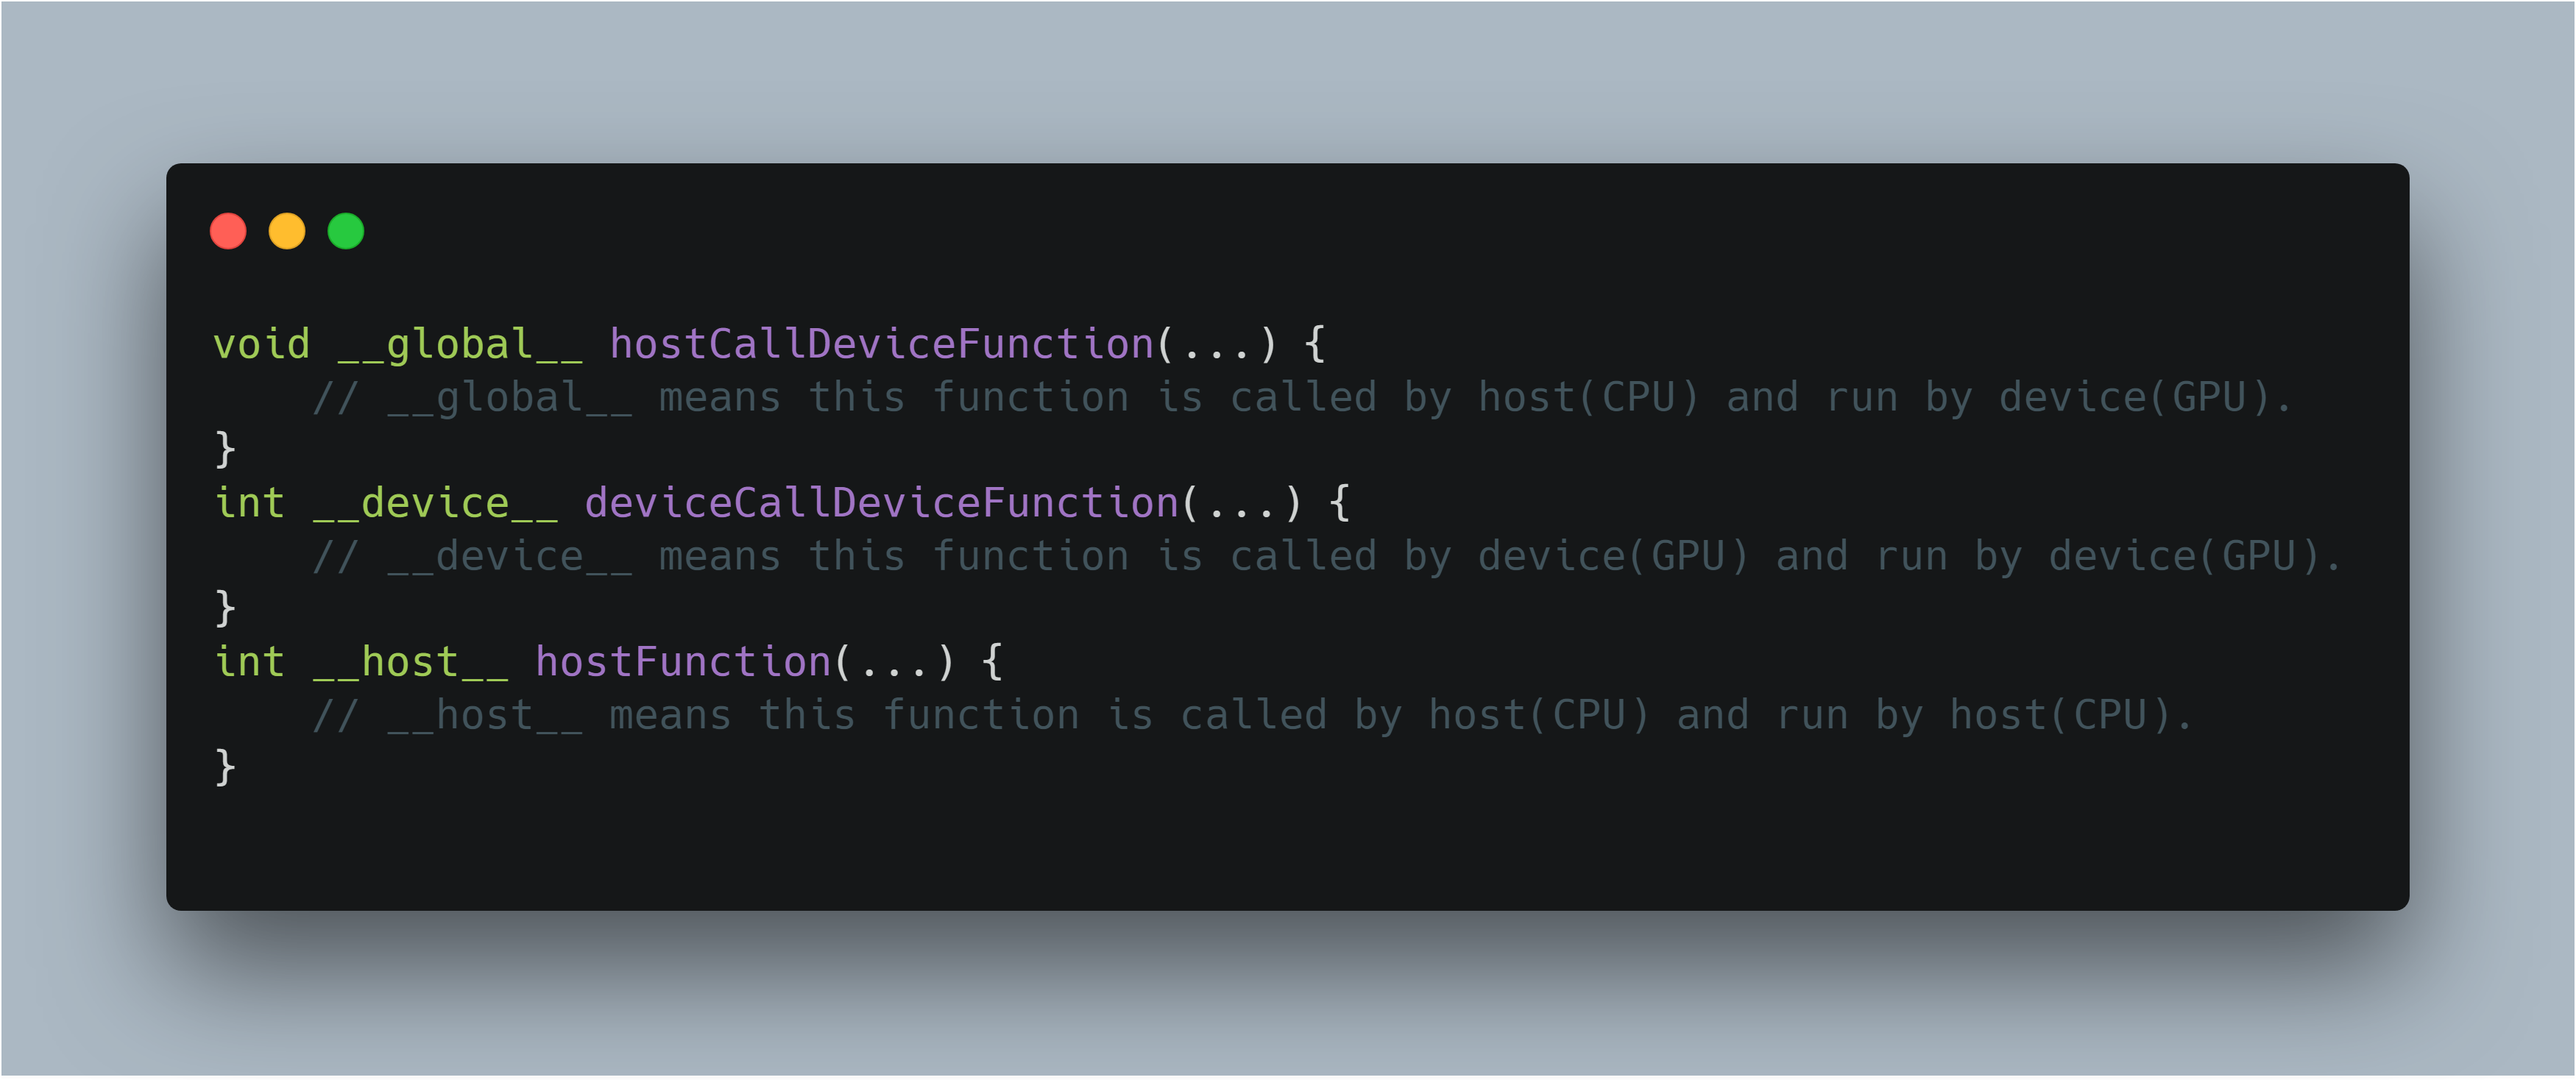
\includegraphics[width=15cm]{figures/CODE1.png}
	\renewcommand{\thefigure}{\arabic{section}-\arabic{figure} }
	\renewcommand{\figurename}{图}
	\caption{CUDA中的三种函数}
	\addtocounter{figure}{-1}
	\renewcommand{\thefigure}{\arabic{section}-\arabic{figure} }
	\renewcommand{\figurename}{Figure}
	\caption{3 types of function in CUDA}
	\label{Fig.2}
\end{figure}
\par 以上代码段加粗部分为CUDA关键字,对于函数有三种修饰:\_\_global\_\_, \_\_device\_\_, \_\_host\_\_. 分别代表被CPU调用运行于GPU、被GPU调用运行于GPU和被CPU调用运行于CPU的函数。其中被CPU调用运行于GPU的函数只能拥有void返回值,且所有运行于GPU的函数都不支持可变参数列表\parencite{EVENEASIER}。\_\_device\_\_和\_\_host\_\_关键字修饰的函数的调用方式与传统函数别无二致,\_\_global\_\_关键字修饰的函数调用方式如图\ref{Fig.4}所示。
\begin{figure}
	\centering
	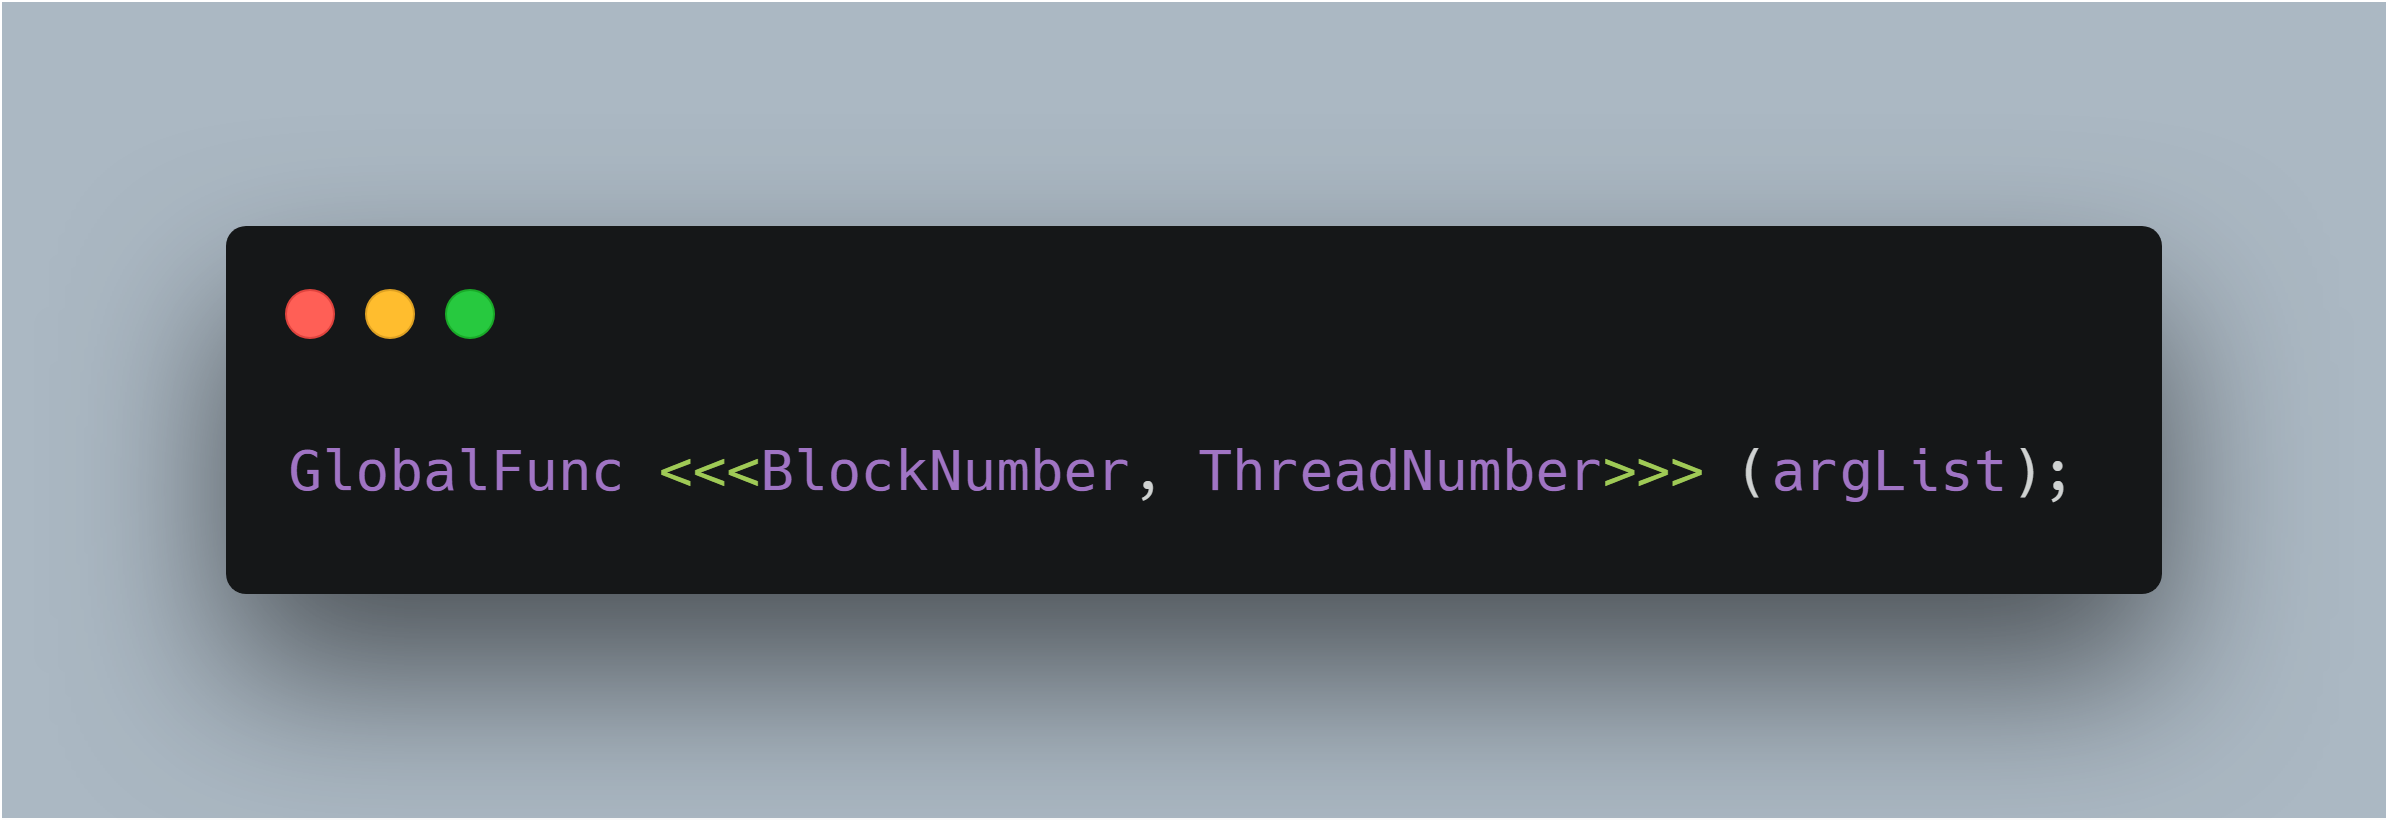
\includegraphics[width=15cm]{figures/CODE3.png}
	\renewcommand{\thefigure}{\arabic{section}-\arabic{figure} }
	\renewcommand{\figurename}{图}
	\caption{CUDA核函数调用方式}
	\addtocounter{figure}{-1}
	\renewcommand{\thefigure}{\arabic{section}-\arabic{figure} }
	\renewcommand{\figurename}{Figure}
	\caption{Invoking method of kernel function in CUDA}
	\label{Fig.4}
\end{figure}
BlockNumber和ThreadNumber分别代表要启动的线程块数目和每个线程块中线程的数目,这一部分取值对程序性能影响较大,之后会详细说明。

\par 之前提到了GPU端的缓存,CUDA程序的另一个重点是存储系统的管理。传统CPU编程模型中,寄存器、缓存等资源都是由CPU自行管理,而不开放给程序员。其原因在于CPU拥有的寄存器、缓存资源较为紧缺,为提高指令级并行能力,需要采用多队列乱序发射与寄存器重命名等技术。相对得,GPU有较为充足的物理寄存器、缓存资源,程序员也对这部分资源掌握有一定的控制权\parencite{CUDAPROG}。CUDA中的存储设备如表\ref{table-存储}所示。
\begin{table}
	\centering
	\renewcommand{\thetable}{\arabic{section}-\arabic{table} }
	\renewcommand{\tablename}{表}
	\caption{CUDA存储系统层级}
	\addtocounter{table}{-1}
	\renewcommand{\thetable}{\arabic{section}-\arabic{table} }
	\renewcommand{\tablename}{Table}
	\caption{CUDA storage system hierarchy}
	\begin{tabular}{cccc}
		\toprule
		项目				&	大小			&	延迟(时钟周期)	&	访问权限	\\
		\midrule
		寄存器文件		&	8KB-64KB/SM		&	$ 10^0 $	& GPU端	\\
		共享内存(L1,L2)	&	16KB-128KB/SM	&	$ 10^1 $	&	GPU端\\
		常量内存		&	N/A				&	N/A		&	N/A	\\
		纹理内存		&	N/A				&	N/A		&	N/A \\
		全局内存		&	-GB				&	$ 10^2 $	&	CPU端/GPU端 \\
		\bottomrule
	\end{tabular} \label{table-存储}
\end{table}
\par 需要注意的是,常量内存与纹理内存都是全局内存的一种虚拟地址形式。和常量内存一样,纹理内存也是一种只读内存;但是在缓存加载的行为方面,常量内存与传统方式一样,加载所访问数据单元的所在行的一部分单元,而纹理内存则加载所访问数据周围一个范围内的单元\parencite{THEDESIGN}。这样做的原因是在GPU进行图形运算时,处理某一像素点需要用到周围一个范围内所有像素点的信息比如进行抗锯齿作业时,而非只有一行,如图\ref{Fig.1}所示。采用这种结构能改善某些访问模式情况下程序的性能。
\par 这些内存的使用方式如图\ref{Fig.3}所示。寄存器和共享内存的使用方式很好理解,关于常量内存和纹理内存,由于他们是全局内存中的虚拟地址,故声明常量内存的语句也就是用了全局内存;纹理内存的使用则需要借助相应API。而一般的全局内存的读写权限同时开放给CPU和GPU,故需要使用特定的API进行访问。
\begin{figure}
	\centering
	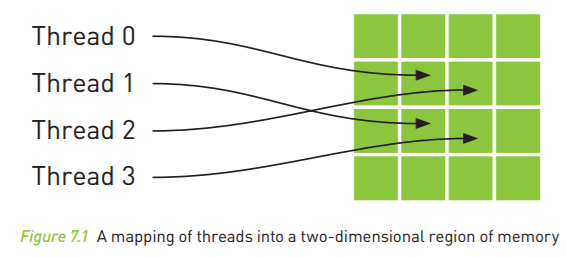
\includegraphics[width=15cm]{figures/Fig1.jpg}
	\renewcommand{\thefigure}{\arabic{section}-\arabic{figure} }
	\renewcommand{\figurename}{图}
	\caption{纹理内存}
	\addtocounter{figure}{-1}
	\renewcommand{\thefigure}{\arabic{section}-\arabic{figure} }
	\renewcommand{\figurename}{Figure}
	\caption{Texture Memory}
	\label{Fig.1}
\end{figure}
\begin{figure}
	\centering
	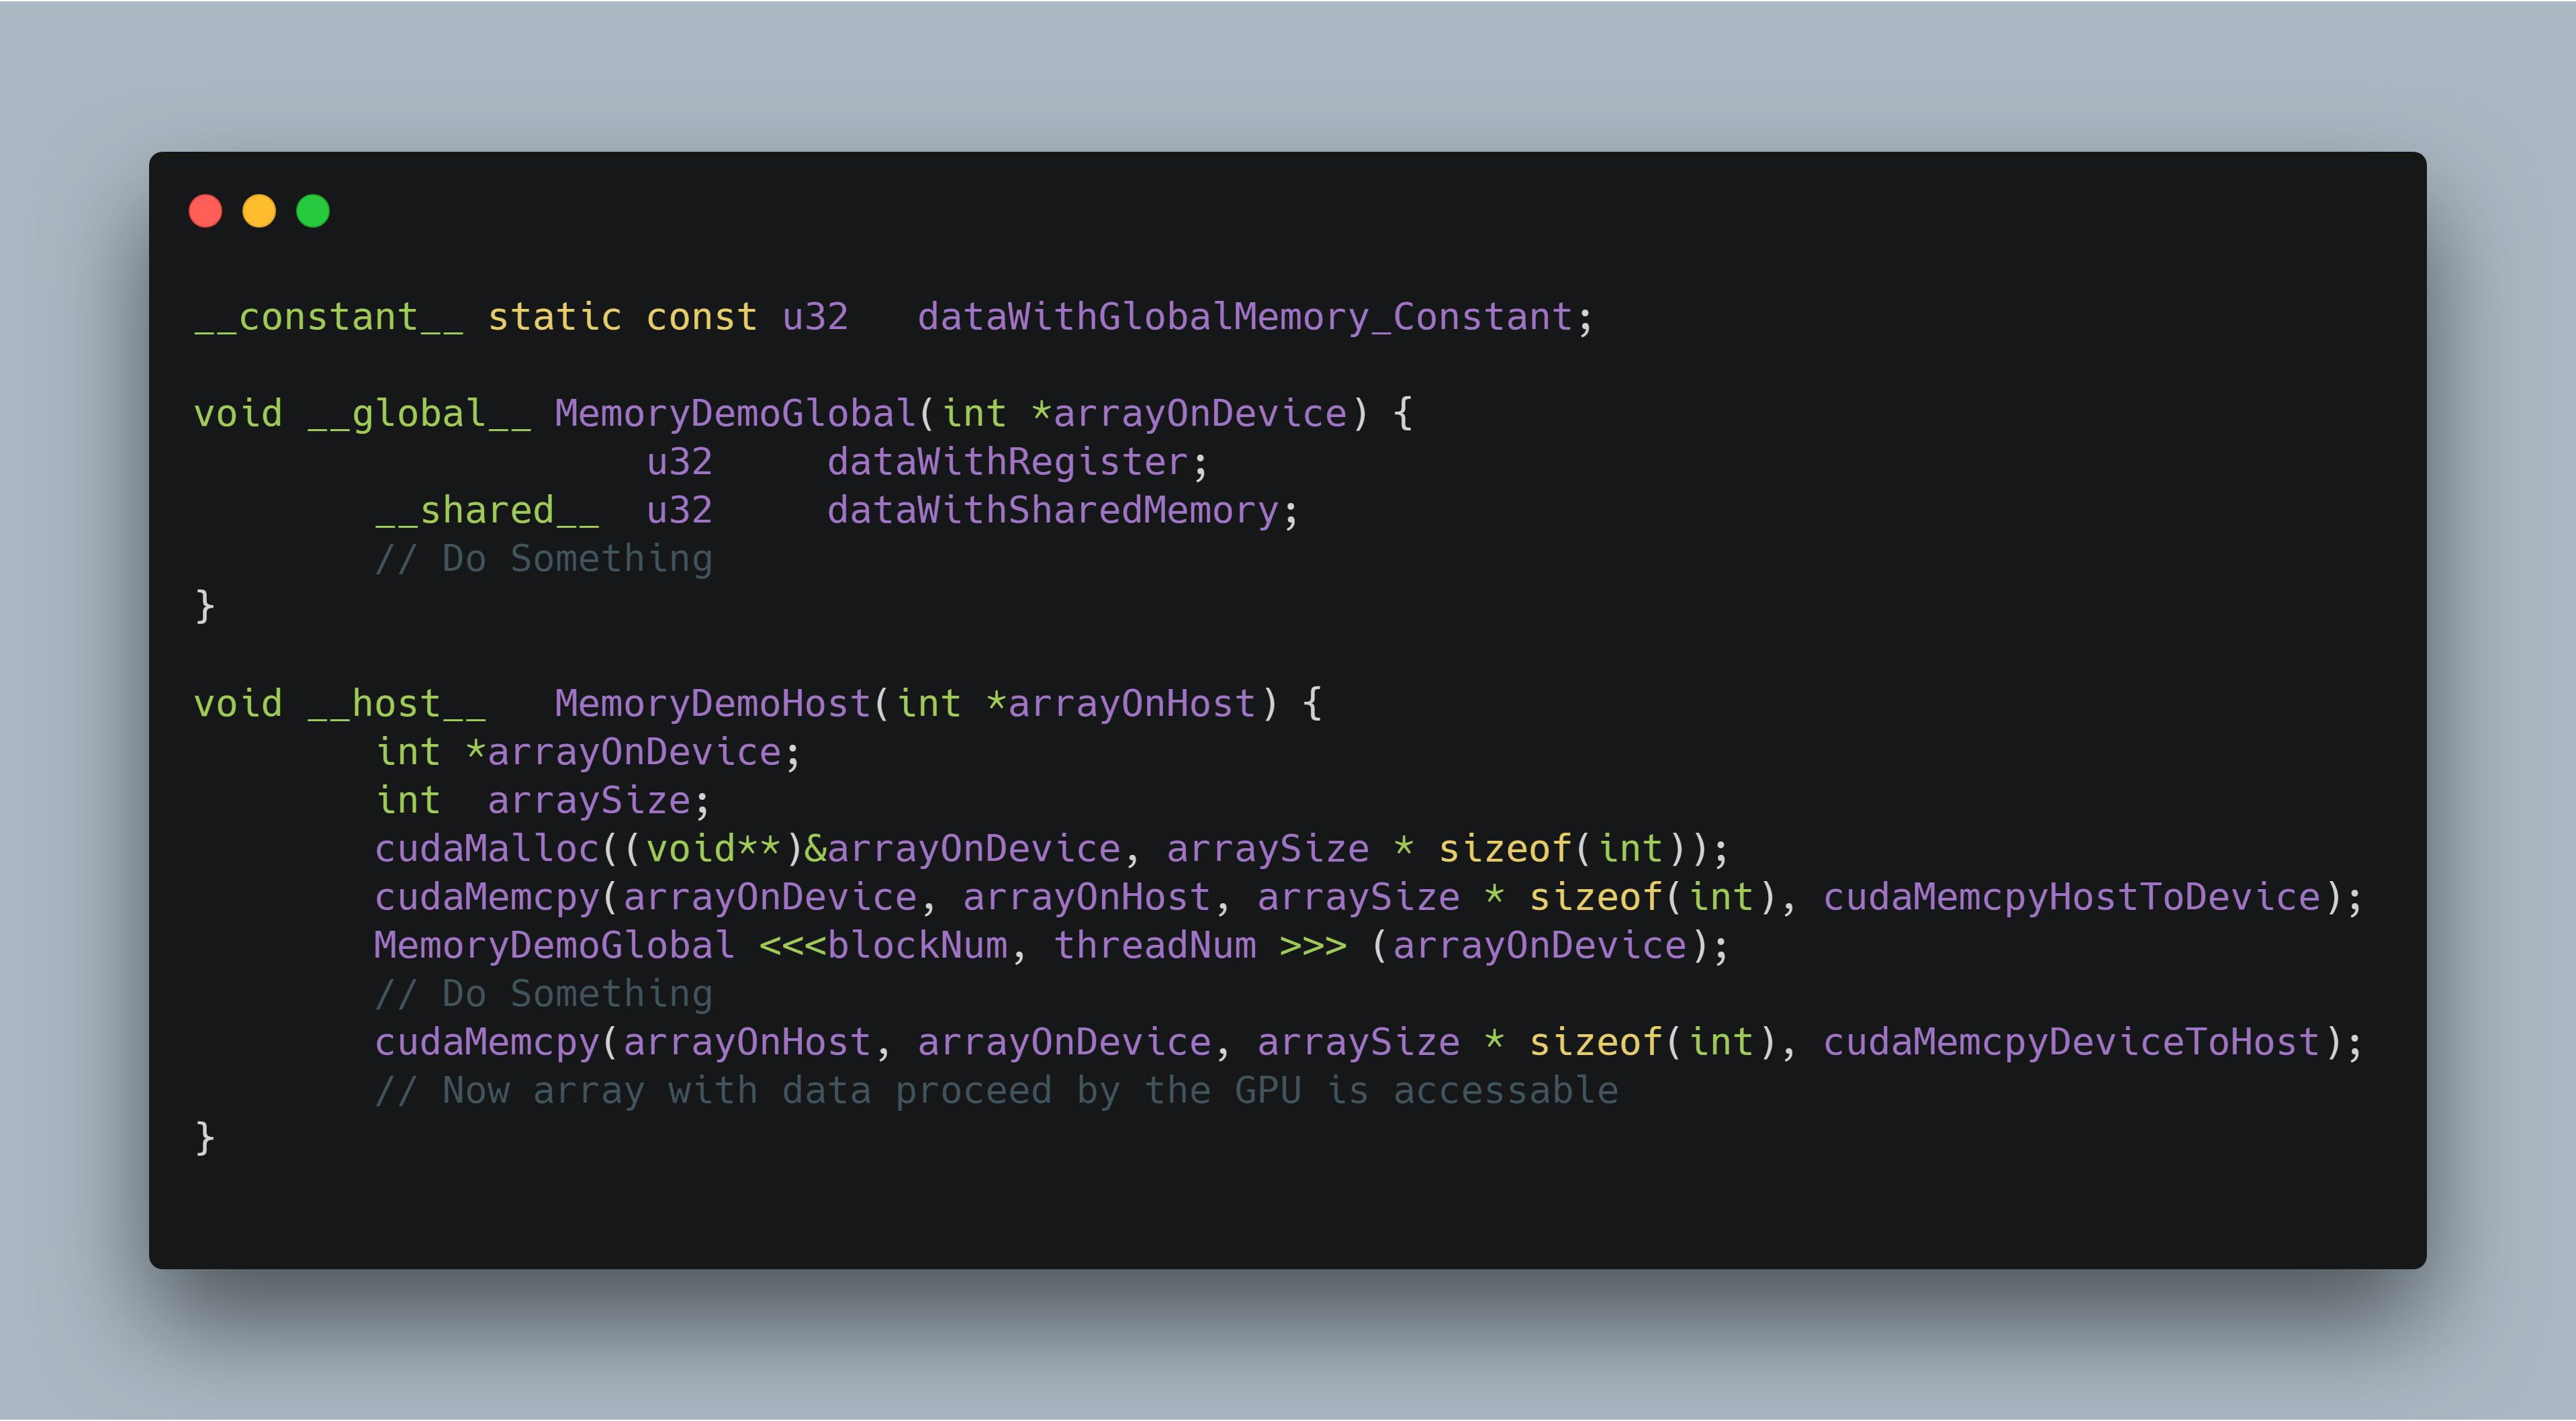
\includegraphics[width=15cm]{figures/CODE2.png}
	\renewcommand{\thefigure}{\arabic{section}-\arabic{figure} }
	\renewcommand{\figurename}{图}
	\caption{不同存储单元的使用方式}
	\addtocounter{figure}{-1}
	\renewcommand{\thefigure}{\arabic{section}-\arabic{figure} }
	\renewcommand{\figurename}{Figure}
	\caption{Methods of using different storage unit}
	\label{Fig.3}
\end{figure}
\paragraph{编译方式}
\par CUDA程序的编译较为简单,只需使用$ nvcc $对源文件进行编译生成可执行文件。首先将从C/C++/CUDA文件编译生成PTX中间代码,再从PTX中间代码生成SASS机器代码。本实验中由于需要观察、研究具体GPU代码的生成方式、特征,故在编译时加入$ --keep $保留编译产生的PTX中间代码文件。而SASS机器代码则在NVIDIA的支持下通过捕捉CUDA应用的指令流获得。
\paragraph{运行模式}
\par 关于如何从CPU端(host)启动GPU端(device)的函数将在下一节通过CPU端应用程序的反汇编代码详细描述,这一节仅介绍GPU相关的部分。
\par 根据弗林分类法\parencite{FLYNN},计算机系统可以分为SIMD, MIMD, SISD, MISD等类型,目前多核心CPU系统就是MIMD系统。而NVIDIA的GPU系统被称为SIMT(单指令多线程),与SIMD(单指令多数据)有所不同。在这种模型中,一条指令并非仅仅代表一个固定的功能,而是代表执行这一指令的类型、使用的管道/流水线。线程需要执行的具体操作需要编写相关内核代码。直观的特征便是再PTX中间代码和SASS机器代码中,所有的逻辑操作指令都是$ lop/lop3 $,通过后缀$ .and/.or, .sync/.async $指明具体运算和调度特征。所以,在SIMT模型中,内核程序读入统一的数据,程序代码根据需要进行不同操作;实际调度时不同操作通过重复指令流按顺序发射,只不过运算单元会屏蔽无关线程。
\par 首先需要介绍一下计算能力,此处计算能力指的是GPU中流多处理器(SM)支持的运算的等级,分为Major和Minor等级,可以等价为流多处理器的代号,所支持的运算不同。其中Major代号代表架构的更新,这也会带来许多新的硬件支持的运算,而Minor代号则代表同一架构下不同定位的流多处理器产品。如伏特架构的计算能力为7.2,图灵架构的计算能力为7.5,Major代号一样就代表这两种架构其实并无太大修改,而Minor代号则代表伏特架构中流多处理器的类型是Heavy,图灵架构中流多处理器的类型是Lite。Lite和Heavy一般用于区分消费级/工作站级GPU,分别对应GeForce和Tesla代号。
\par 基于GPU的应用与传统的基于CPU的应用在运行方式上有较大差别,主要有以下几点。
\begin{itemize}
	\item GPU中由大量的物理寄存器,达几十~几百KB,且都能在1个时钟周期内访问,而CPU中物理寄存器资源极为有限。故在进行上下文切换时,GPU只需更改寄存器文件指针来切换,而CPU需要使用堆栈保存上下文。
	\item CPU仅仅支持数十个硬件线程,而GPU则支持数千个硬件线程。在GPU上开启过少的硬件线程会极大降低硬件使用率,进而导致性能降低。具体开启线程数量取决于硬件SM最大并发线程数、最大并发线程束数和最大并发块数等。表\ref{table-占用率}显示了在不同计算能力上开启不同数量的线程时设备的利用率以及所能开启包含该数量线程的线程块的数量。\\
	\begin{table}
	\centering
	\renewcommand{\thetable}{\arabic{section}-\arabic{table} }
	\renewcommand{\tablename}{表}
	\caption{可分配线程数与占用率的关系}
	\addtocounter{table}{-1}
	\renewcommand{\thetable}{\arabic{section}-\arabic{table} }
	\renewcommand{\tablename}{Table}
	\caption{Available thread number and corresponding occupancy rate}
	\begin{tabular}{cccccc}
		\toprule
			&	1.0	&1.2	&2.0	&2.1	&3.0 \\
		\midrule
		64	&	67\%, 8		&	50\%, 8		&	33\%, 8		&	33\%, 8		&	50\%, 16	\\
		96	&	100\%, 8	&	75\%, 8		&	50\%, 8		&	50\%, 8		&	75\%, 12	\\
		128	&	100\%, 6	&	100\%, 8	&	67\%, 8		&	67\%, 8		&	100\%, 10	\\
		256	&	100\%, 3	&	100\%, 4	&	100\%, 6	&	100\%, 6	&	100\%, 8	\\
		512	&	67\%, 1		&	100\%, 2	&	100\%, 2	&	100\%, 3	&	100\%, 4	\\
		1024&	N/A, N/A	&	N/A, 1		&	67\%, 1		&	67\%, 1		&	100\%, 2	\\
		
		\bottomrule
	\end{tabular} \label{table-占用率}
	\end{table}
	可见,随着计算能力的增长,一个流多处理器上所能容纳的线程束月俩月多。在充分利用寄存器文件和共享内存(L1缓存)的情况下开启线程数越多,设备利用率越高。然而过多的线程会导致资源紧缺,在实际使用中应当根据硬件参数,问题规模做出调整。
\end{itemize}
\par 在CUDA程序中,32个线程被组织成一个线程束(warp),作为基本的调度单元,具有各自的物理寄存器,也就是说线程束中32个线程一般情况下都会执行相同指令流,为SIMD模式。在目前的图灵架构中,线程束仍然是同步的单位,即线程束之间可以保证同步,线程束内部线程无法保证同步。在下一代安培架构(Ampere)则引入$ Arrive-Wait $模式以实现线程级别同步,以提高CUDA程序的灵活性。 
\par 若干个线程束被组织为一个线程块(block),在下一代安培架构中将添加一个线程束组的层级(warp group),由四个线程束组成,但该层级仅为大规模通用矩阵乘法运算所用(Ultra MMA),且本代架构还未应用,这里不做讨论。线程块中的线程束可以通过\_\_syncthread()进行同步,线程块中的线程能够访问共享内存进行数据交换。一个线程块被分配在一个流多处理器上执行,一个流多处理器能分配多个线程块。
\par 若干个线程块被组织成一个线程网格(grid),线程网格可被看作一个分配给GPU的任务。
\par 表\ref{table-粒度}详细说明了CUDA应用中不同不同粒度的线程组织形式。
\begin{table}
	\centering
	\renewcommand{\thetable}{\arabic{section}-\arabic{table} }
	\renewcommand{\tablename}{表}
	\caption{线程组织形式}
	\addtocounter{table}{-1}
	\renewcommand{\thetable}{\arabic{section}-\arabic{table} }
	\renewcommand{\tablename}{Table}
	\caption{Type of organizing threads}
	\begin{tabular}{ccc}
		\toprule
		粒度	&	调度者	& 	分配给 \\
		\midrule
		warp		&	流多处理器内部调度器	&	流处理器(Stream Processor)\\
		block(CTA)	&	TPC调度器(MPC)		  &		流多处理器(Stream Multi-processor)\\
		grid		&	GPC调度器(GPM)		  &		TPC(Texture Processing Cluster)$ * $\\
		kernel		&	CPU, PCIe			&		GPC(Graphics Processing Cluster)	\\	
		\bottomrule
	\end{tabular} \label{table-粒度}\\

$ * $ 在本世代图灵架构及以前,TPC与SM可以等价,因为一个TPC上仅包含一个SM,然而自下一代安培架构开始,一个TPC中将会有若干个SM。虽然本文研究的图灵架构的硬件在逻辑上SM与TPC等价,但在硬件上还是会做区分,故在表中详细写出\parencite{BLOCKDIAG}。
\end{table}
\par 以上内容介紹了CUDA中的线程组织形式,接下来将介绍调度方式。一个任务也可被看作一个线程网格,由CPU分配该GPU上的GPC,在线程块级别的调度上,GPU将遵循负载均衡的原则在某一线程块工作结束释放资源时调度下一线程块。在线程级别的调度上,一般情况下将以32个线程为单位进行调度,这32个线程执行同一指令流处理不同数据流;而在产生分支时,与CPU使用分支预测处理分支指令,遇到预测错误则清空流水线不同,GPU采用线程束分化(CBU指令)的方式处理;线程束分化机制下每一个分支都会有线程执行到,在分支结束处聚合。对于不满足分支条件的线程,GPU调度器将这些线程设置为未激活状态,继续向下执行。然而,硬件调度器每周期只能为一个线程束取到一条指令,这意味着线程束中部分线程会被阻塞,从而导致利用率下降,性能下降。在编写程序时,应尽量避免线程束内部线程分化,而在CUDA中存在非常细致的线程、线程块、线程网格ID,故根据这些ID控制分支使得线程束内部线程分化尽可能少时可行的\parencite{DIVER}。自麦克斯韦架构(Maxwell)以来,指令集中添加了CBU(Convergence Barrier Unit)指令以保持通过同一分支的线程被组织在一起,就是为了减少线程束分化带来的性能下降\parencite{THREADS}。
\par 最后将介绍CUDA中流这一机制以及相应的锁页内存。CUDA流可被看作一个GPU操作队列,该队列中的操作将会按顺序执行,这一特点使得在实际编写程序的过程中可以通过调整不同操作的顺序,如访存、密集的计算、写会等来隐藏数据依赖和控制依赖带来的延迟\parencite{STREAM},通过异步操作(ASYNC)提升任务级并行度。CUDA流需要在支持设备重叠的GPU上运行。设备重叠只GPU能够在执行一个核函数时在设备和主机间进行数据交互。
\par 而为了支持CUDA流,所有涉及流的内存需要字啊锁页内存上进行分配。锁页内存正如其字面含义,是分配在显存上、不允许被移动或被换页到磁盘上的设备内存。其好处是允许GPU上的DMA控制器绕过CPU直接请求主机传输数据,在延迟更低的基础上支持设备重叠。若不适用锁页内存,DMA控制器在定位内存页面时会造成困难。本文中,TensorRT中利用了CUDA流的特性,将在相应章节介绍。
\par 这一章从线程组织形式到调用运行方式介绍了CUDA应用,对实验中进行设备相关的优化有较大的帮助。
\subsection{目前展开的工作}
\par 本文的研究同时涉及硬件和软件:Nvidia新架构的GPU与使用GPU加速计算的机器学习应用,注意这里的机器学习应用并不只是现在大行其道的深度学习,还包括传统的基于概率模型的方法等。
\par 在近年来深度学习迅猛发展之前,关于使用GPU并行化机器学习算法的研究就已有很多,甚至可以说正是基于GPU的强大并行计算能力,深度学习才能发展如此迅速。早在2005年,D. Steinkraus等人便对在GPU上实现机器学习算法进行了研究, 当时实现的算法是OCR,如今OCR能够非常快速、方便地通过各种框架、语言实现。然而这一研究奠定了使用GPU加速机器学习应用的基础\parencite{GPUFORML}。之后的几年中,除去OCR外,基于GPU的各种并行机器学习算法包括kNN\parencite{KNNG},支持向量机\parencite{SMOSVM}都慢慢成熟。由于贝叶斯网络的精确推理是个NP难的问题,其性能受限于硬件水平,然而根据Md Vasimuddin等人的研究\parencite{BAYESINF},通过并行方法将延迟降低了许多。由于传统机器学习方法有着延迟低、模型小、训练时间短、可解释性强等优点,在深度学习迅猛发展的今天,传统机器学习方法仍然占有很大的市场,故评估GPU对传统机器学习加速的性能是十分有必要的。本文中在评估传统机器学习的部分便采用了并行的支持向量机算法(SMO-SVM),如今,不管是在工业生产领域还是学术研究领域,该算法仍占有一席之地。
\par 之后不久,深度学习、神经网络便迎来了爆炸式的发展。实际上在二十世纪末,便已经有完整的神经网络算法的理论基础;在1979年,日本学者福岛邦彦提出了Neocognition模型,其中使用多层网络以及神经元对图像特征进行提取和筛选被认为是启发了卷积神经网络的开创性研究\parencite{JAPANESSAY}。1989年,LeCun首次在论文中提出了“卷积”一次,卷积神经网络因此得名\parencite{LENET}。在1993年,贝尔实验室对LeCun的工作进行了代码实现,并大量部署于手写支票识别系统,然而限于当时计算能力低下,基于神经网络的研究也停滞在了理论阶段,其主要原因便是网络中需要训练的参数太多,网络结构复杂,在当时没有芯片能满足如此高的性能要求\parencite{NNML}。然而,随着高性能GPU芯片的出现,基于神经网络的方法正如日中天地发展。从TinyCNN等较轻量级、功能单一的库,到TensorFlow、PyTorch、Caffe、Chain等完整、易于使用的框架,这些工具或是本身就是基于GPU编写的,或是慢慢更新对GPU的支持;目前市面上的绝大部分该类产品均支持使用GPU运行,单单使用CPU进行深度学习训练已经成为历史。在本文中,卷积神经网络由于它的广泛性、高性能、典型性,在本文中被选为深度学习部分评估的主要载体。
\par 而准确地对GPU以及机器学习的性能进行评估也尤为重要。且为了深入研究GPU对于机器学习应用的性能提升的幅度以及不同提升幅度的不同原因,单单是对训练时间进行统计、评估是不够的。因本文涉及Nvidia新架构GPU中新加入的硬件以及对应CUDA中新加入的API等,故指令、运行流级别的分析是有必要的。Ali Bakhoda等人曾设计实现了一种在软件层面对CUDA执行流进行指令级别的模拟和仿真的系统GPGPU-SIM,该系统是基于Kepler架构的硬件以及CUDA 3.0版本,在缓存命中率、分支、指令乱序执行等方面能达到90-95\%与真实硬件的吻合程度\parencite{GPGPUSIM}。在之后Mahmoud Khairy等人对该系统进行了改进,使其支持伏特架构(Volta)的GPU以及对应的CUDA 9.0 \parencite{GPGPUSIM2}。然而,目前GPU硬件已经更新到图灵架构(Turing),基于安培架构(Ampere)的硬件也即将发布;对应的CUDA版本已经更新到了10.1,在指令执行、调度方式等方面都发生了很多的改变;且Mahmoud Khairy等人的工作主要着重于GPU的内存等方面。故能够准确评估新硬件的系统非常必要。本文中选用了nvprof、NSight等公开的工具,这些工具能从指令运行时间、访存、缓存命中率等方面对CUDA应用程序进行评估\parencite{NSIGHT}。
\par 在新架构的GPU中,最为重要的便是新加入的计算单元:张量核心(Tensor Core),该运算单元能为深度神经网络中大量存在的张量计算带来明显的提升\parencite{VOLTAWHITEPAPER},然而这些数据是Nvidia官方白皮书中给出的数据,开发者社区中反映很少有情况能获得如Nvidia官方宣传所能得到的性能提升;而关于Tensor Core的研究少之又少,故本文并非旨在填补这方面研究的空白,姑且在新的方向进行一些稚嫩的尝试;且由于在Nvidia进行实习工作,有机会接触到许多内部资料,本文是一个很好的契机。
\par 当然,仅有理论计算性能的研究是无力的,最终本文还是会回归实际,使用实际应用中的模型,如各种结构的神经网络、广泛使用的支持向量机并行库对新架构的GPU进行评估。从广为各大厂商使用的深度学习性能评估工具DeepBench\parencite{DEEPBENCH},到使用cudnn从C++源码实现的卷积神经网络,再使用Tensor Flow框架实现的各种结构的网络,包括LeNet-5\parencite{LENET},ResNet\parencite{RESNET},MobileNet\parencite{MOBILE}等,本文将由下而上对新架构硬件再浮点精度计算、张量计算、卷积计算、矩阵计算等方面进行评估,不求全面,只求能给出启发。

\subsection{CUDA应用的汇编代码与PTX中间代码的结构}

\subsubsection{CUDA应用汇编代码结构}
\begin{figure}
	\centering
	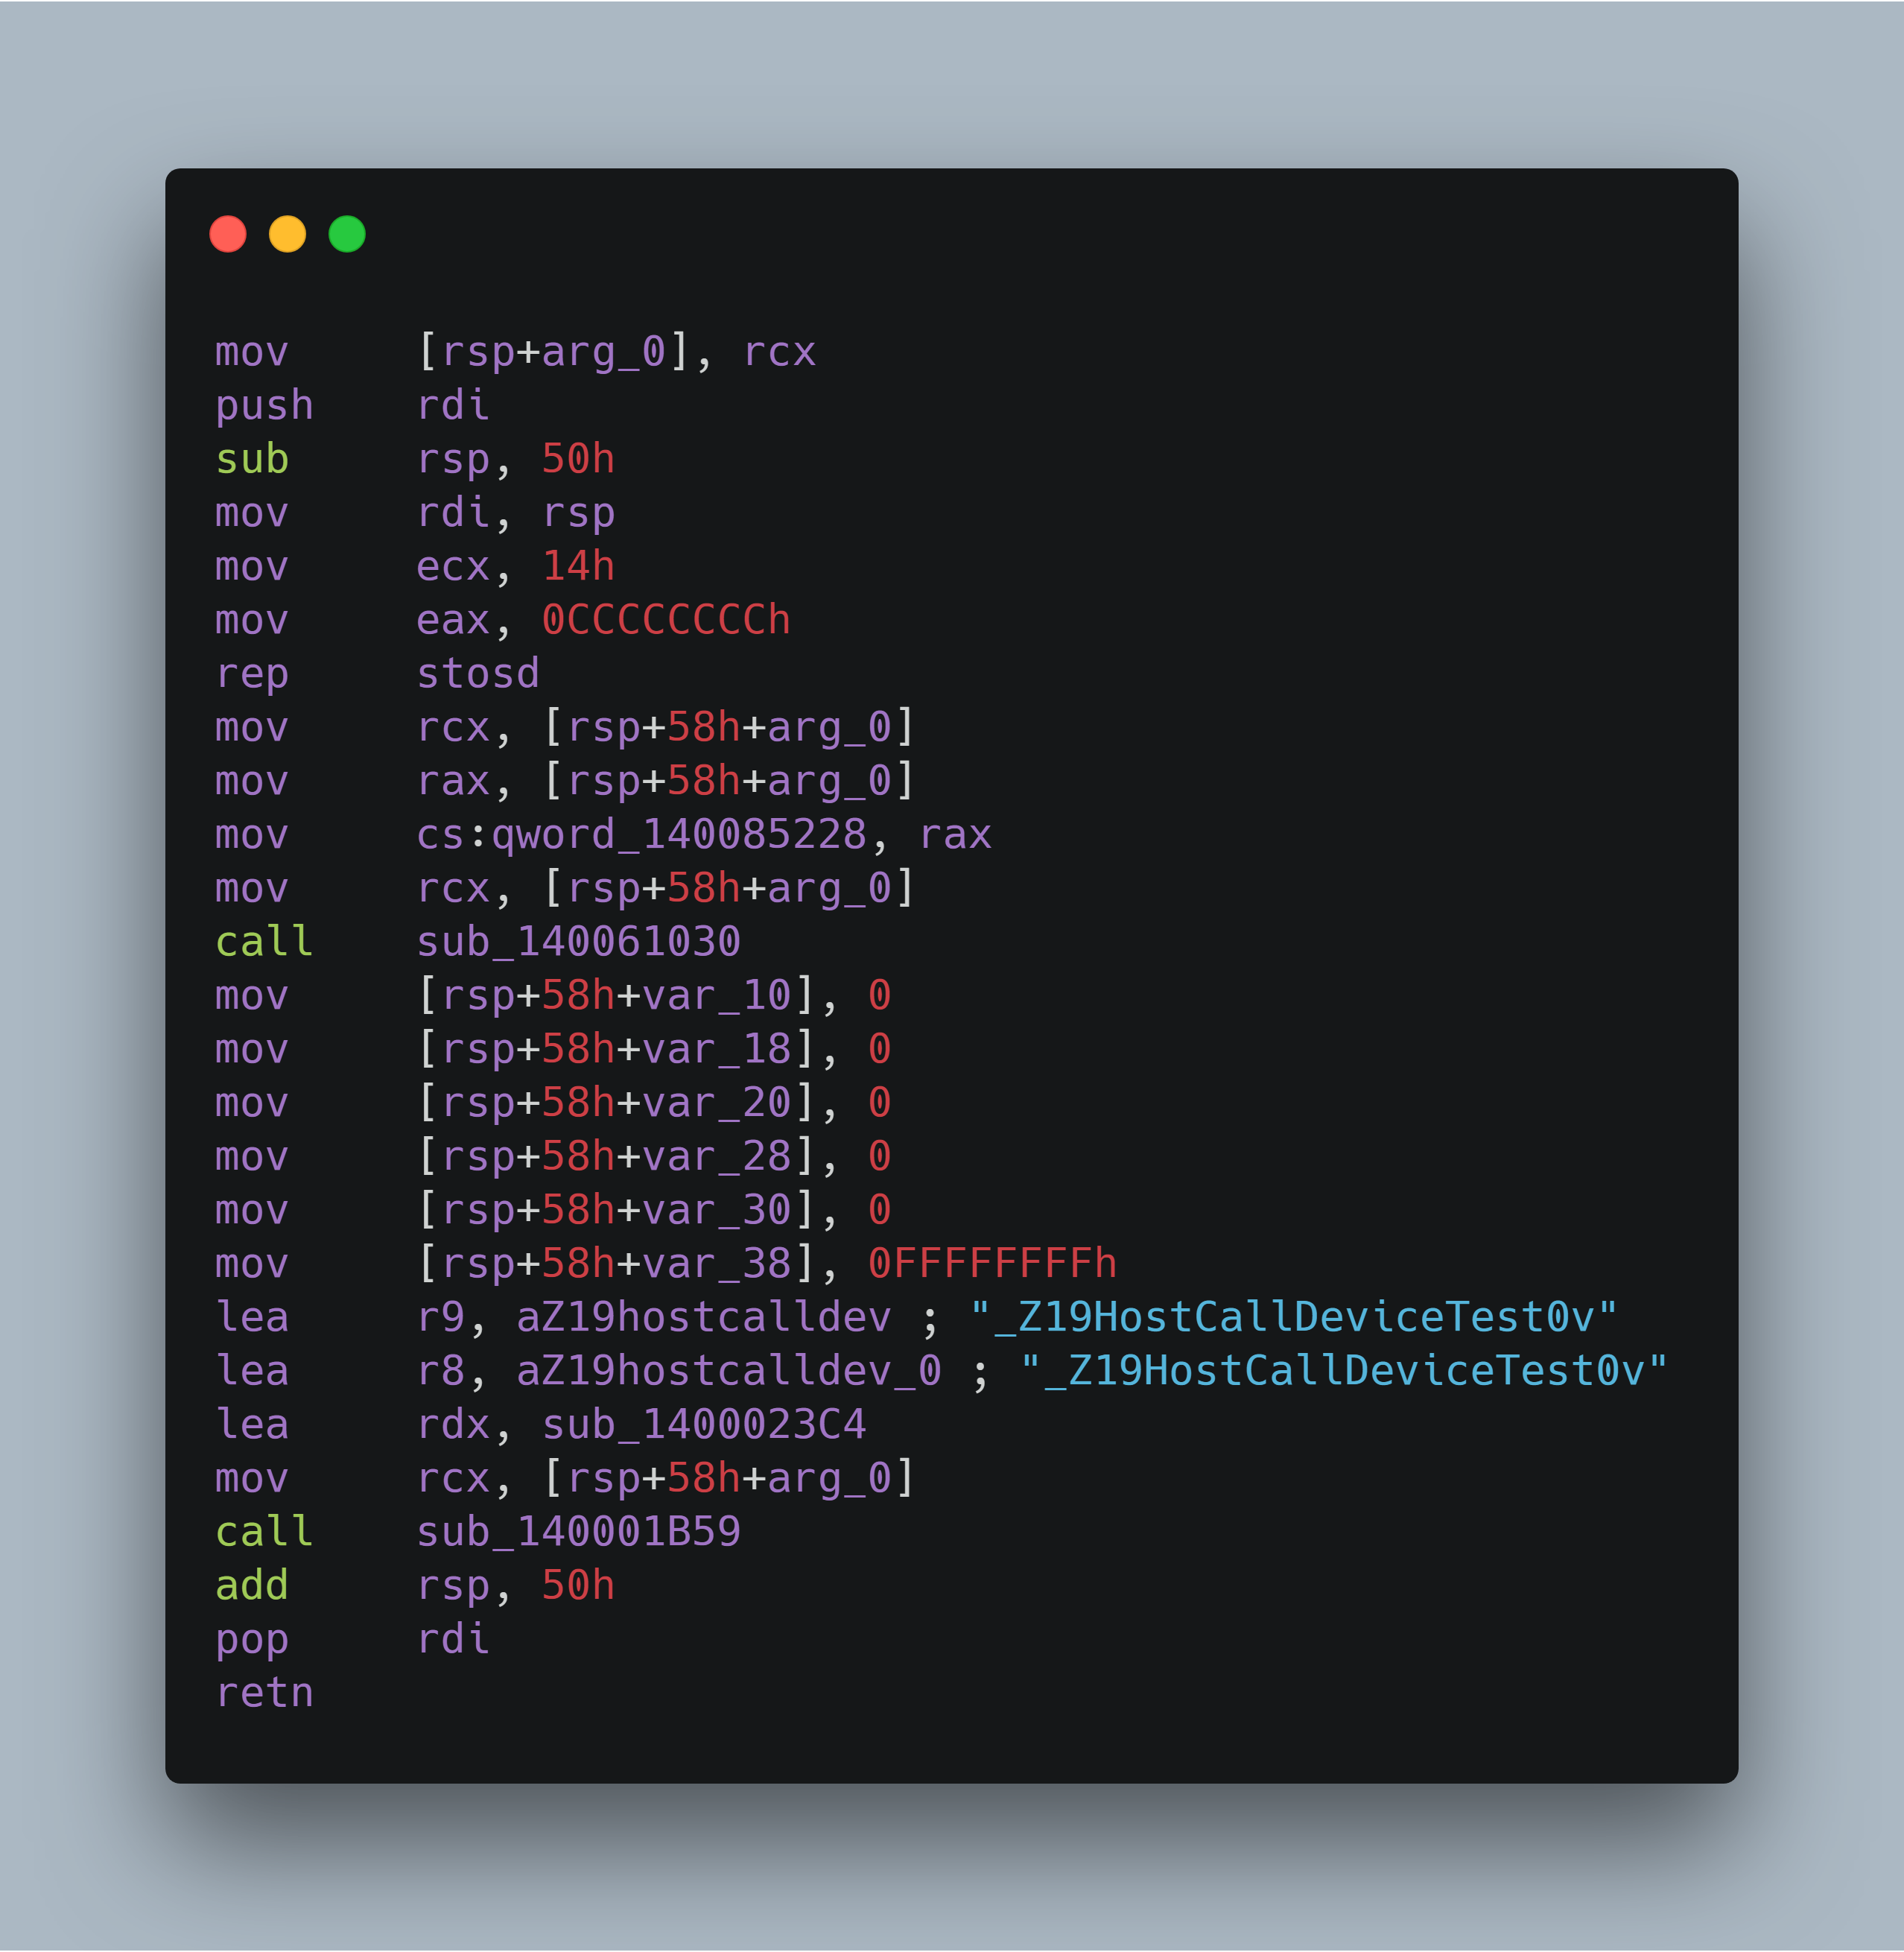
\includegraphics[width=15cm]{figures/CODE4.png}
	\renewcommand{\thefigure}{\arabic{section}-\arabic{figure} }
	\renewcommand{\figurename}{图}
	\caption{CUDA程序部分反汇编代码}
	\addtocounter{figure}{-1}
	\renewcommand{\thefigure}{\arabic{section}-\arabic{figure} }
	\renewcommand{\figurename}{Figure}
	\caption{Part of assembly code of CUDA application}
	\label{Fig.CUDA-Assembly}
\end{figure}
\par 这一节通过CUDA程序在x86\_64架构的CPU下使用静态反汇编生成的汇编代码说明涉及运行于GPU的核函数的调用与返回方式、控制权转交方式等。
\begin{itemize}
\item CUDA中三种函数只有被\_\_global\_\_修饰的函数在讨论范围内,因为只有这种函数跨越CPU与GPU,该函数被称为内核函数(Kernel Function)。调用核函数的加载过程与核函数的地址被存储在数据区(仅有核函数地址,因核函数实际运行于GPU)。
\item 主函数需要定位到核函数加载过程,将核函数加载过程的地址通过lea指令加载进相关寄存器(rcx或rdx),该过程并非被call指令直接调用。
\item 进入加载过程,在执行一系列堆栈检查后,使用call指令调用传递CUDA函数执行时$ <<< >>> $中参数的过程。
\item 正式将核函数地址使用lea指令加载进相关寄存器(r8、r9),然后使用call指令调用正式调用过程,该过程中还包含一系列安全性检查,核函数执行控制权交予GPU,如图\ref{Fig.CUDA-Assembly}所示。
\item 因调用核函数时并非用call指令直接调用,而是使用lea指令加载地址进入寄存器,故CPU端不会等待核函数返回,而是直接执行之后的函数或语句。
\item \_\_device\_\_修饰的函数调用都在PTX代码中。
\end{itemize}

\subsubsection{PTX中间代码结构} %正文第二章
\newpage
\section{评估NVIDIA新架构GPU的机器学习应用性能}
\setcounter{table}{0}
\setcounter{figure}{0}
\subsection{实验工具与环境}
\subsubsection{实验环境}
\par 表\ref{table-环境}中列出实验环境。\\
\begin{table}
	\centering
	\renewcommand{\thetable}{\arabic{section}-\arabic{table} }
	\renewcommand{\tablename}{表}
	\caption{实验环境}
	\addtocounter{table}{-1}
	\renewcommand{\thetable}{\arabic{section}-\arabic{table} }
	\renewcommand{\tablename}{Table}
	\caption{Environment}
	\begin{tabular}{cc}
		\toprule
		项目	&	内容\\
		\midrule
		CPU		&	AMD Ryzen ThreadRipper 2990WX 32C64T @ 3.0GHz\\
		主板		&	MSI X399\\
		内存		&	CORSAIR DDR4 3200 @ 16-15-15-15-34-1T 128GB\\
		GPU		&	NVIDIA Geforce RTX 2080TI (Turing)\\
		硬盘		&	INTEL750 NVMe PCIe 1.2TB * 2 @ RAID 0\\
		系统		&	Windows 10 64-bit build 17763\\	
		CUDA	&	10.1, 10.0, 9.2, 9.0\\
		其他		&	Jetson TX2 $ * $\\
		\bottomrule
		$ * $该硬件由NVIDIA提供。\\
	\end{tabular} 
	\label{table-环境}
\end{table}

\subsubsection{实验工具}
\par 实验中使用到了若干软件工具,如表\ref{table-实验工具}列出。
\begin{table}
	\centering
	\renewcommand{\thetable}{\arabic{section}-\arabic{table} }
	\renewcommand{\tablename}{表}
	\caption{实验工具}
	\addtocounter{table}{-1}
	\renewcommand{\thetable}{\arabic{section}-\arabic{table} }
	\renewcommand{\tablename}{Table}
	\caption{Tools}
	\begin{tabular}{cc}
		\toprule
		项目	&	内容\\
		\midrule
		Python 3.6		&	用于进行数据统计、编写TensorFlow应用\\
		Conda 4.5.12		&	用于创建、管理、隔离Python环境\\
		TensorFlow		&	1.12.0和1.13.0版本的源码,用于对比、研究、调整\\
		Bazel 0.16.0		&	用于从源码构建TensorFlow\\
		Msys2		&	用于从源码构建TensorFlow\\
		CMake 3.1.0		&	用于构建CUTLASS\\	
		Nsight 6.0	&	用于后台监听CUDA应用,捕捉Trace\\
		nvprof		&	用于分析CUDA程序的API调用、分支效率等\\
		git			&	版本控制\\
		Perforce	&	版本控制\\
		Ubuntu 16.04 Physical & 用于执行GPGPU-SIM 应用\\
		GPGPU-SIM 3.2 & 用于从指令级别模拟CUDA程序\\
		Visual Studio 2017 & 搭配10.0.17763.0版本的SDK\\
		\bottomrule
	\end{tabular} \label{table-实验工具} 
\end{table}
\subsection{实验详细过程}
\subsubsection{基于测试样例的Benchmark}
\par 为了为接下来的实验设定基准,这一步先使用用途单一的测试样例测试绝对性能以及相应的提升,因不同架构的硬件各项参数(包括流处理器数量、显存容量等)不尽相同,所以直接对比不同架构硬件的性能是没有意义的,这里选择对比不同架构硬件在不同SDK下性能提升的比例。此处选用了CUDA 10.0,CUDA 9.2,CUDA 9.0三种SDK,同时选用9.2与9.0的原因是因为9.2版本是为了图灵架构的GPU Tesla V100发布的\parencite{CUDA92},也在本文的研究范围内。
\par 因为本文主要讨论新架构GPU在机器学习应用中带来的性能提升,故选用的评测样例大部分都与机器学习应用相关;主要从以下角度进行评估:通用矩阵乘法(GEMM, General Matrix Multiply)、矩阵乘法运算性能、卷积运算性能、神经网络推理性能以及结合框架的综合性能。在评估这些性能时也会包含单/双精度浮点计算性能。
\paragraph{通用矩阵乘法(GEMM, General Matrix Multiply)}
\subparagraph{实验结果}
\par 根据开发者社区的反映,新架构硬件性能的差别主要体现在问题规模、问题类型等方面(张量维度、形状,训练/推理任务等),而NVIDIA官方仅给出一种规模的结果,所以本节使用了自行编写的一系列测试用例,辅以深度学习测试套件DeepBench\parencite{DEEPBENCH},在开启和关闭新架构中张量核心的情况下进行测试。实验性能使用TFlops/s统计,方法为简单的运算数除以运算时间,运算时间的统计采用CUDA内置的$ cudaEvent $记录。
\par 首先评估的是在不同问题规模下,开启和关闭新架构中的张量核心所能达到的性能,如图\ref{Fig-PerfGemm}所示。随着问题规模的上升,总体加速比呈上升趋势,在大规模数据时半精度通用矩阵运算性能的加速比能达到3到3.5倍、单精度通用矩阵运算性能的加速比能达到2倍。然而,单纯考察数据规模发现加速比差距非常大,甚至是在大规模数据中仍然存在开启张量核心后性能不如不开启张量核心的情况,结合文档在通用矩阵运算一章中在指令中需要指明运算的最小单元这一点中\parencite{PTX};可以推测出输入矩阵的“形状”对张量核心的性能由较大影响。
\par 为了研究输入矩阵“形状”对于加速比的影响,由于两个输入矩阵涉及三个维度,故采用控制变量法,控制$ m,n,k $中某一维度考察另外两个维度对于加速比的影响。由于测试数据中存在部分离群值($ N\geq 500000 $),这会对作图精度产生极大影响,故先予以剔除。实验结果如图\ref{Fig-MNKRatio}所示。可见在两个输入矩阵的三个维度中,两矩阵共享的维度$ K $对于性能的影响最为显著。
\par 关于矩阵的形状、维度对于性能的影响,其原因将在后文结果分析中详细说明。以上实验数据以及性能旨在考查开启和关闭张量核心时性能提升幅度,故开启的线程块数量和线程数量较小,相应的GPU占用率也较小,导致所得性能并非GPU峰值性能。为测量峰值性能,这里还是用NVIDIA官方发布的用于线性代数计算的模板库CUTLASS(CUDA Template Linear Algebra Subroutines),该模板库根据新架构硬件特性编写,提供了许多测试样例供参考,这里使用CUTLASS测试得到的性能作为峰值性能基准。
\par CUTLASS库中的GEMM运算有多种精度可供选择:HGEMM、SGEMM、DGEMM、CGEMM、ZGEMM和IGEMM,分别代表半精度浮点、单精度浮点、双精度浮点、单精度复数、双精度复数和八位整数。鉴于之前的测试并不涉及复数,此处也不选用复数精度作为基准。需要注意的是测试样例后缀中存在$ \_[n/t][n/t] $分别代表运算中输入矩阵的数据存储、分布方式,即行列是否转置(如上文提到的,CUDA中矩阵存储分行主元素和列主元素存储)。图\ref{Fig-GEMM-CUTLASS}为测得的性能基准。
\begin{figure}
	\centering
	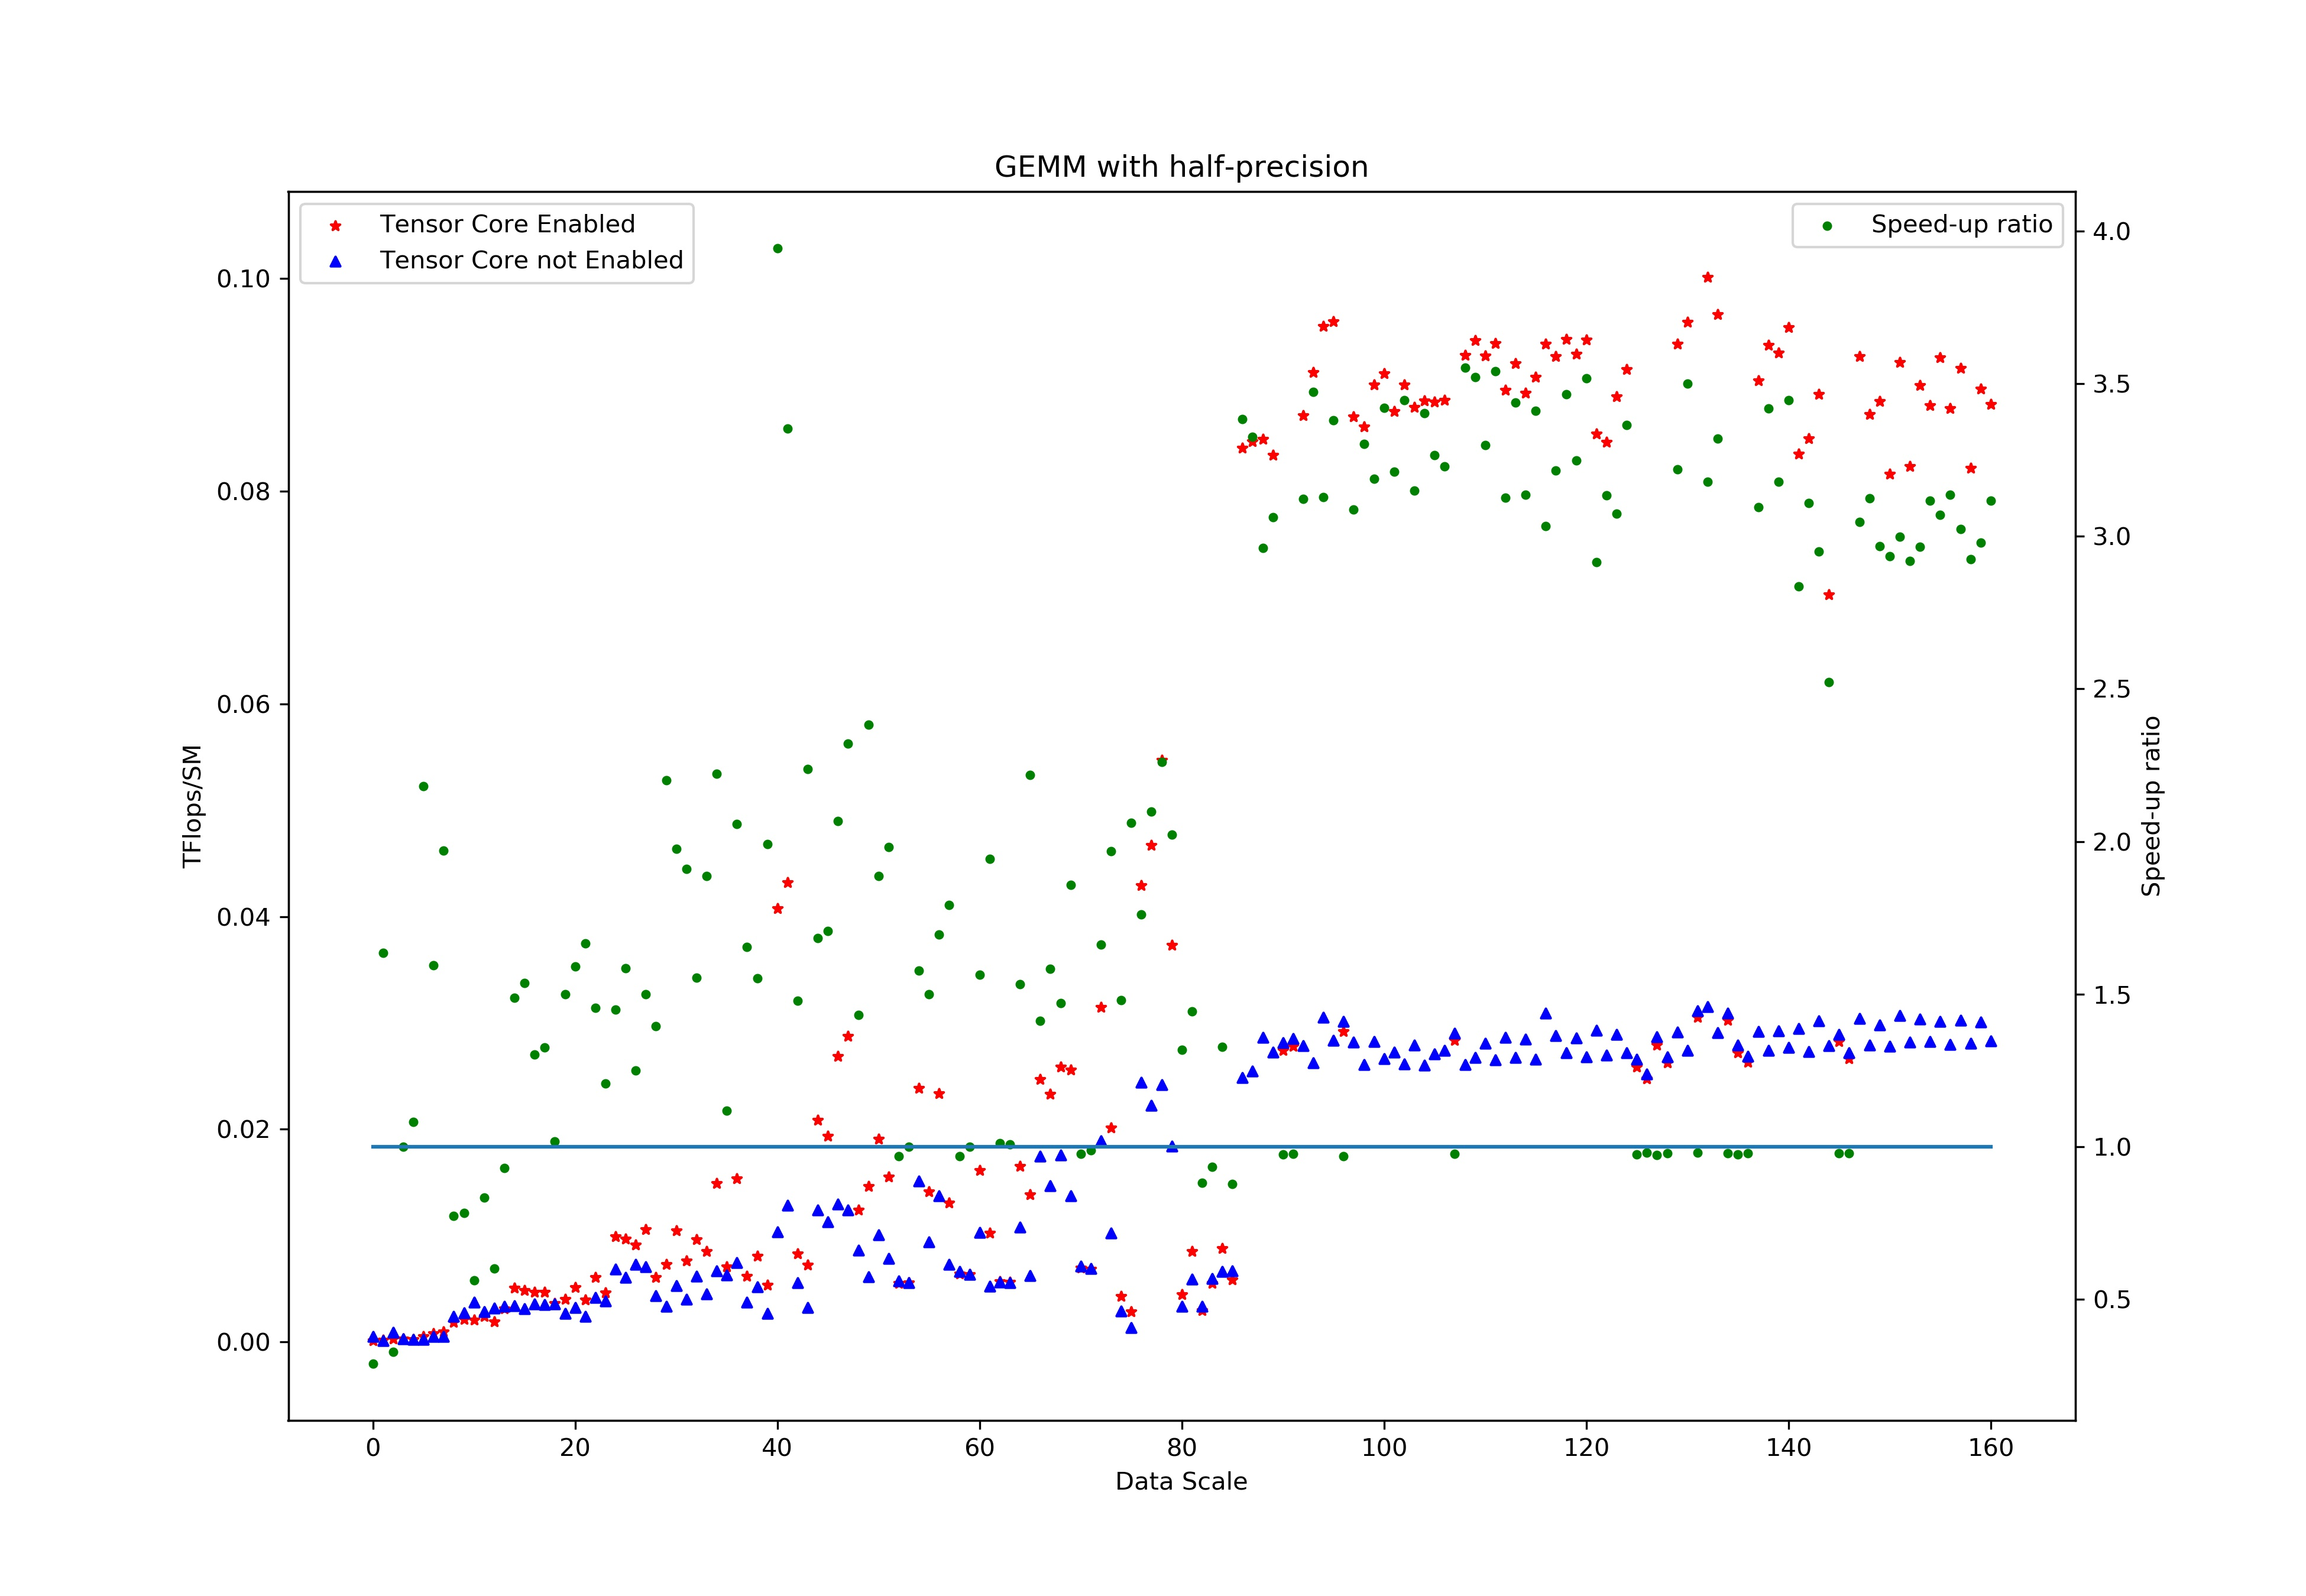
\includegraphics[width=7.5cm]{figures/GEMM-Half-TF.jpg}
	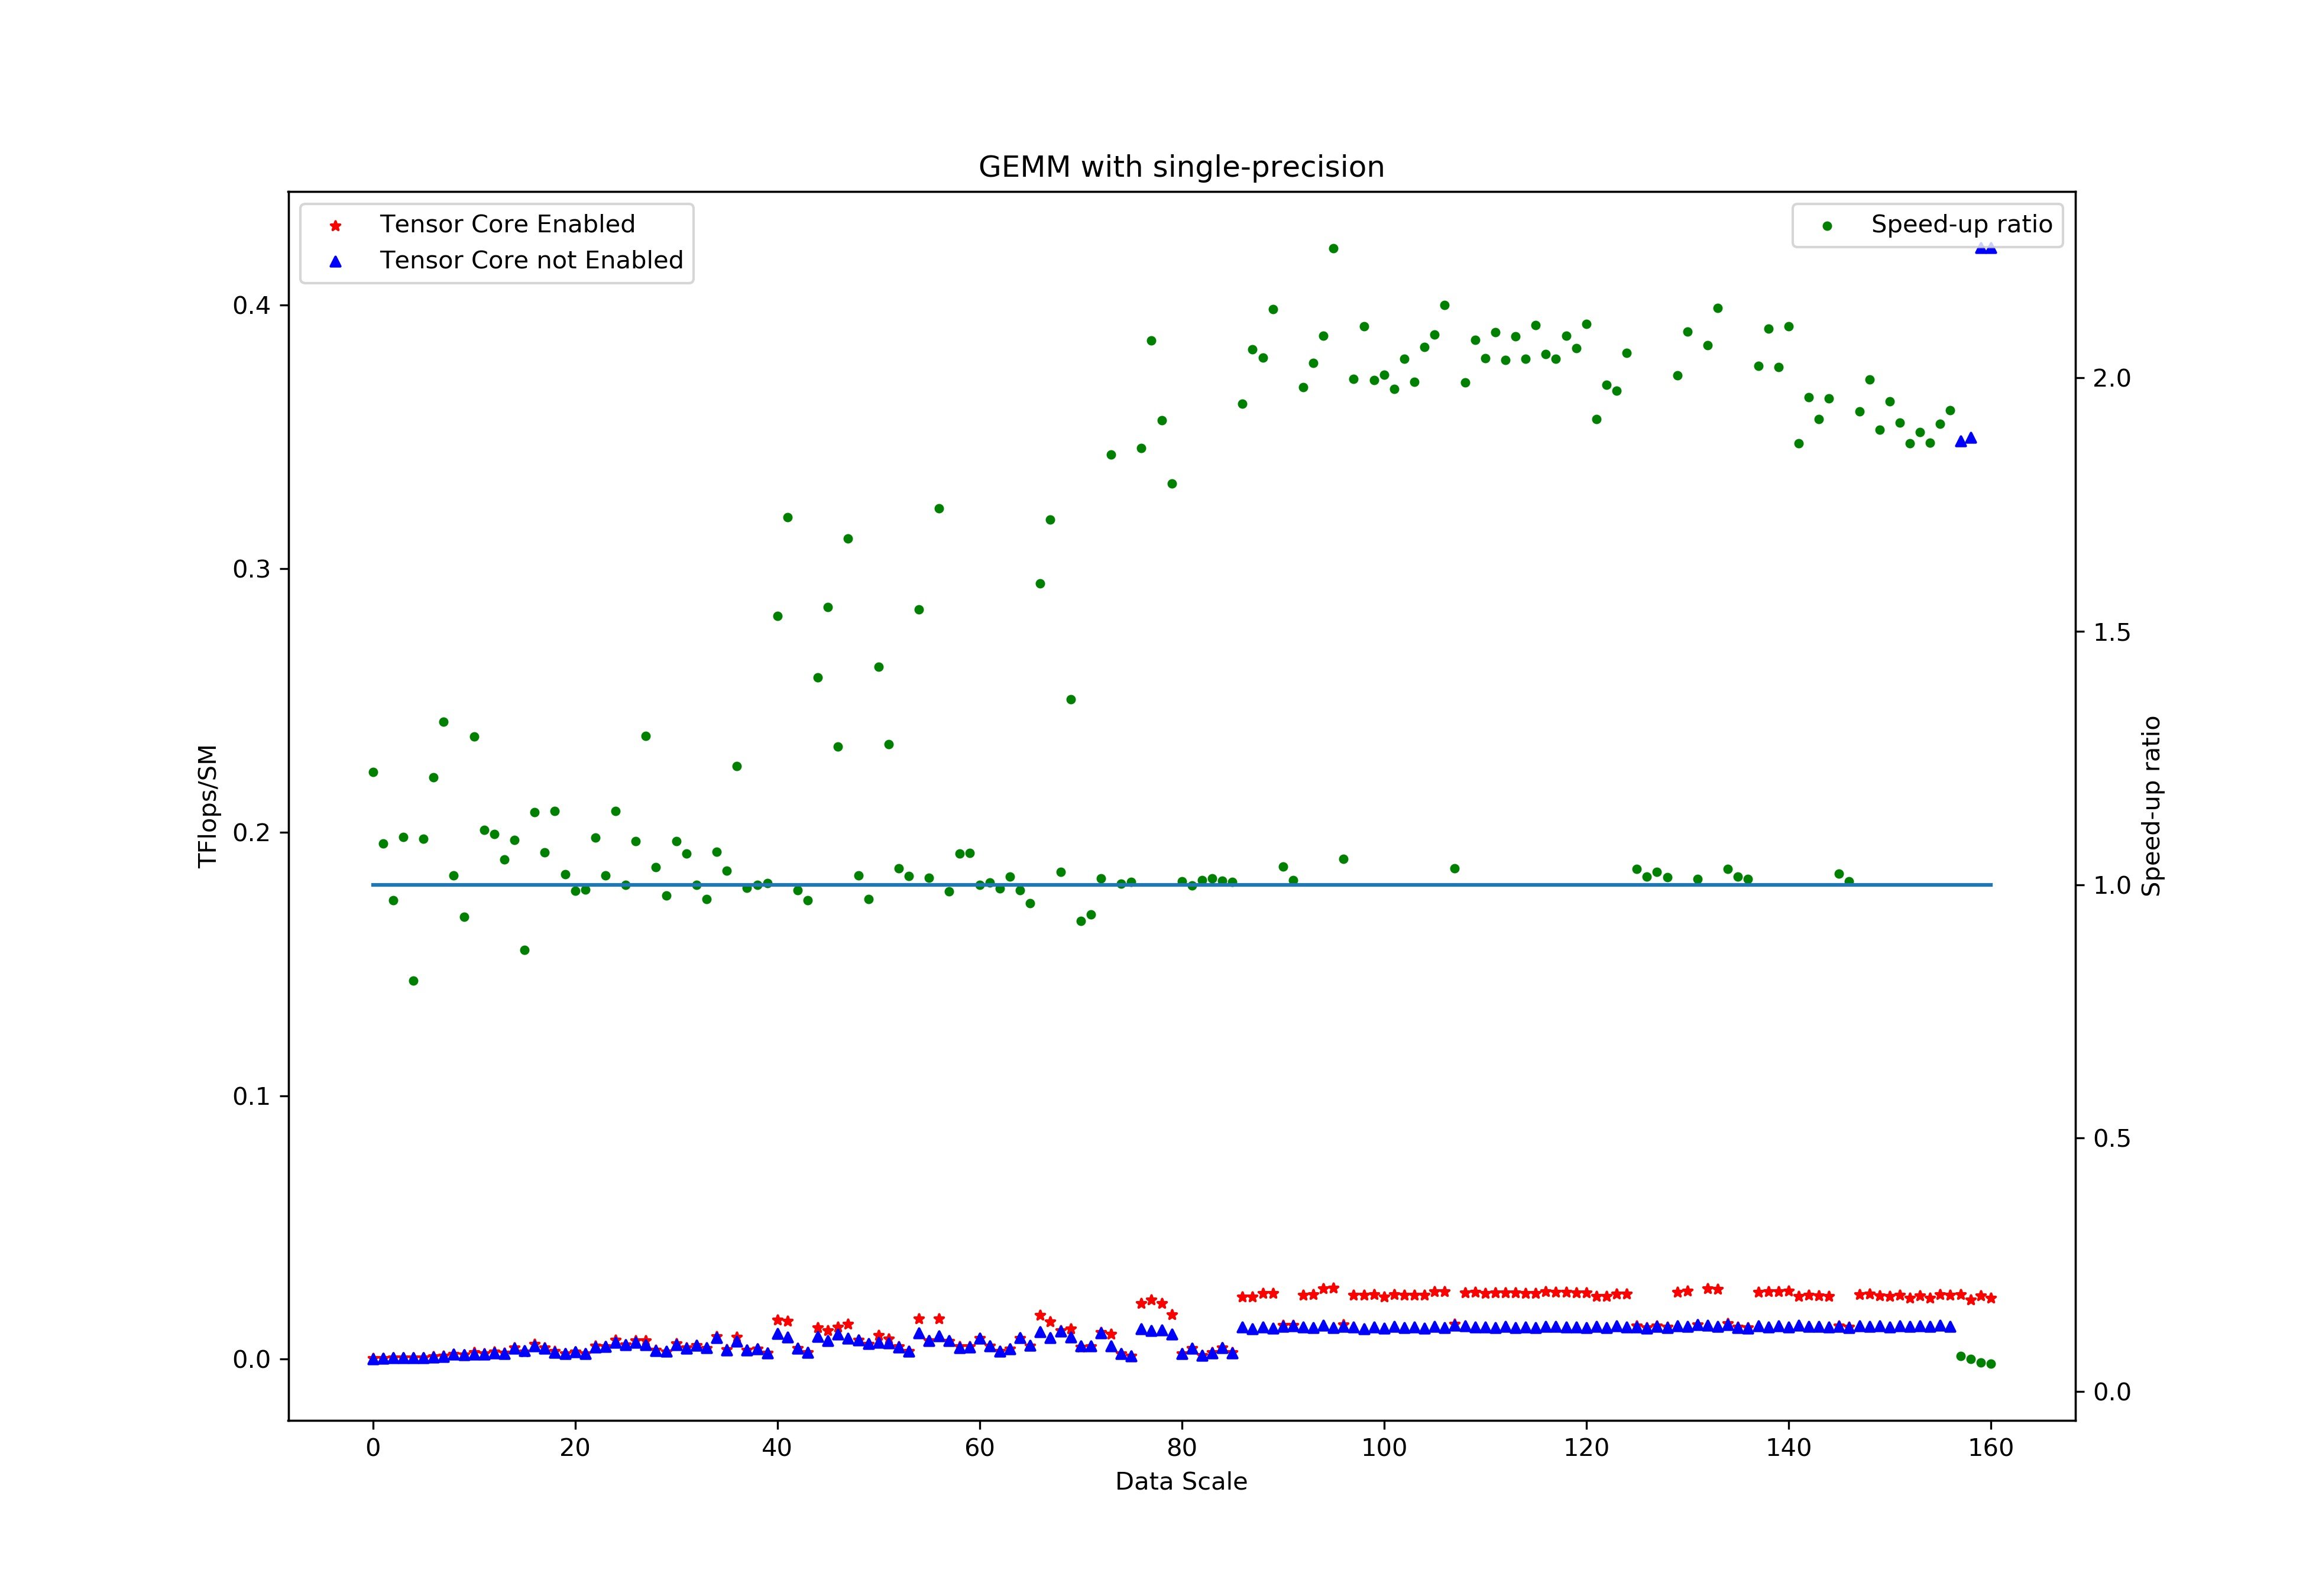
\includegraphics[width=7.5cm]{figures/GEMM-Single-TF.jpg}
	\renewcommand{\thefigure}{\arabic{section}-\arabic{figure} }
	\renewcommand{\figurename}{图}
	\caption{半精度/单精度GEMM性能}
	\addtocounter{figure}{-1}
	\renewcommand{\thefigure}{\arabic{section}-\arabic{figure} }
	\renewcommand{\figurename}{Figure}
	\caption{Performance of GEMM at Half and Single}
	\label{Fig-PerfGemm}
\end{figure}
\begin{figure}
	\centering
	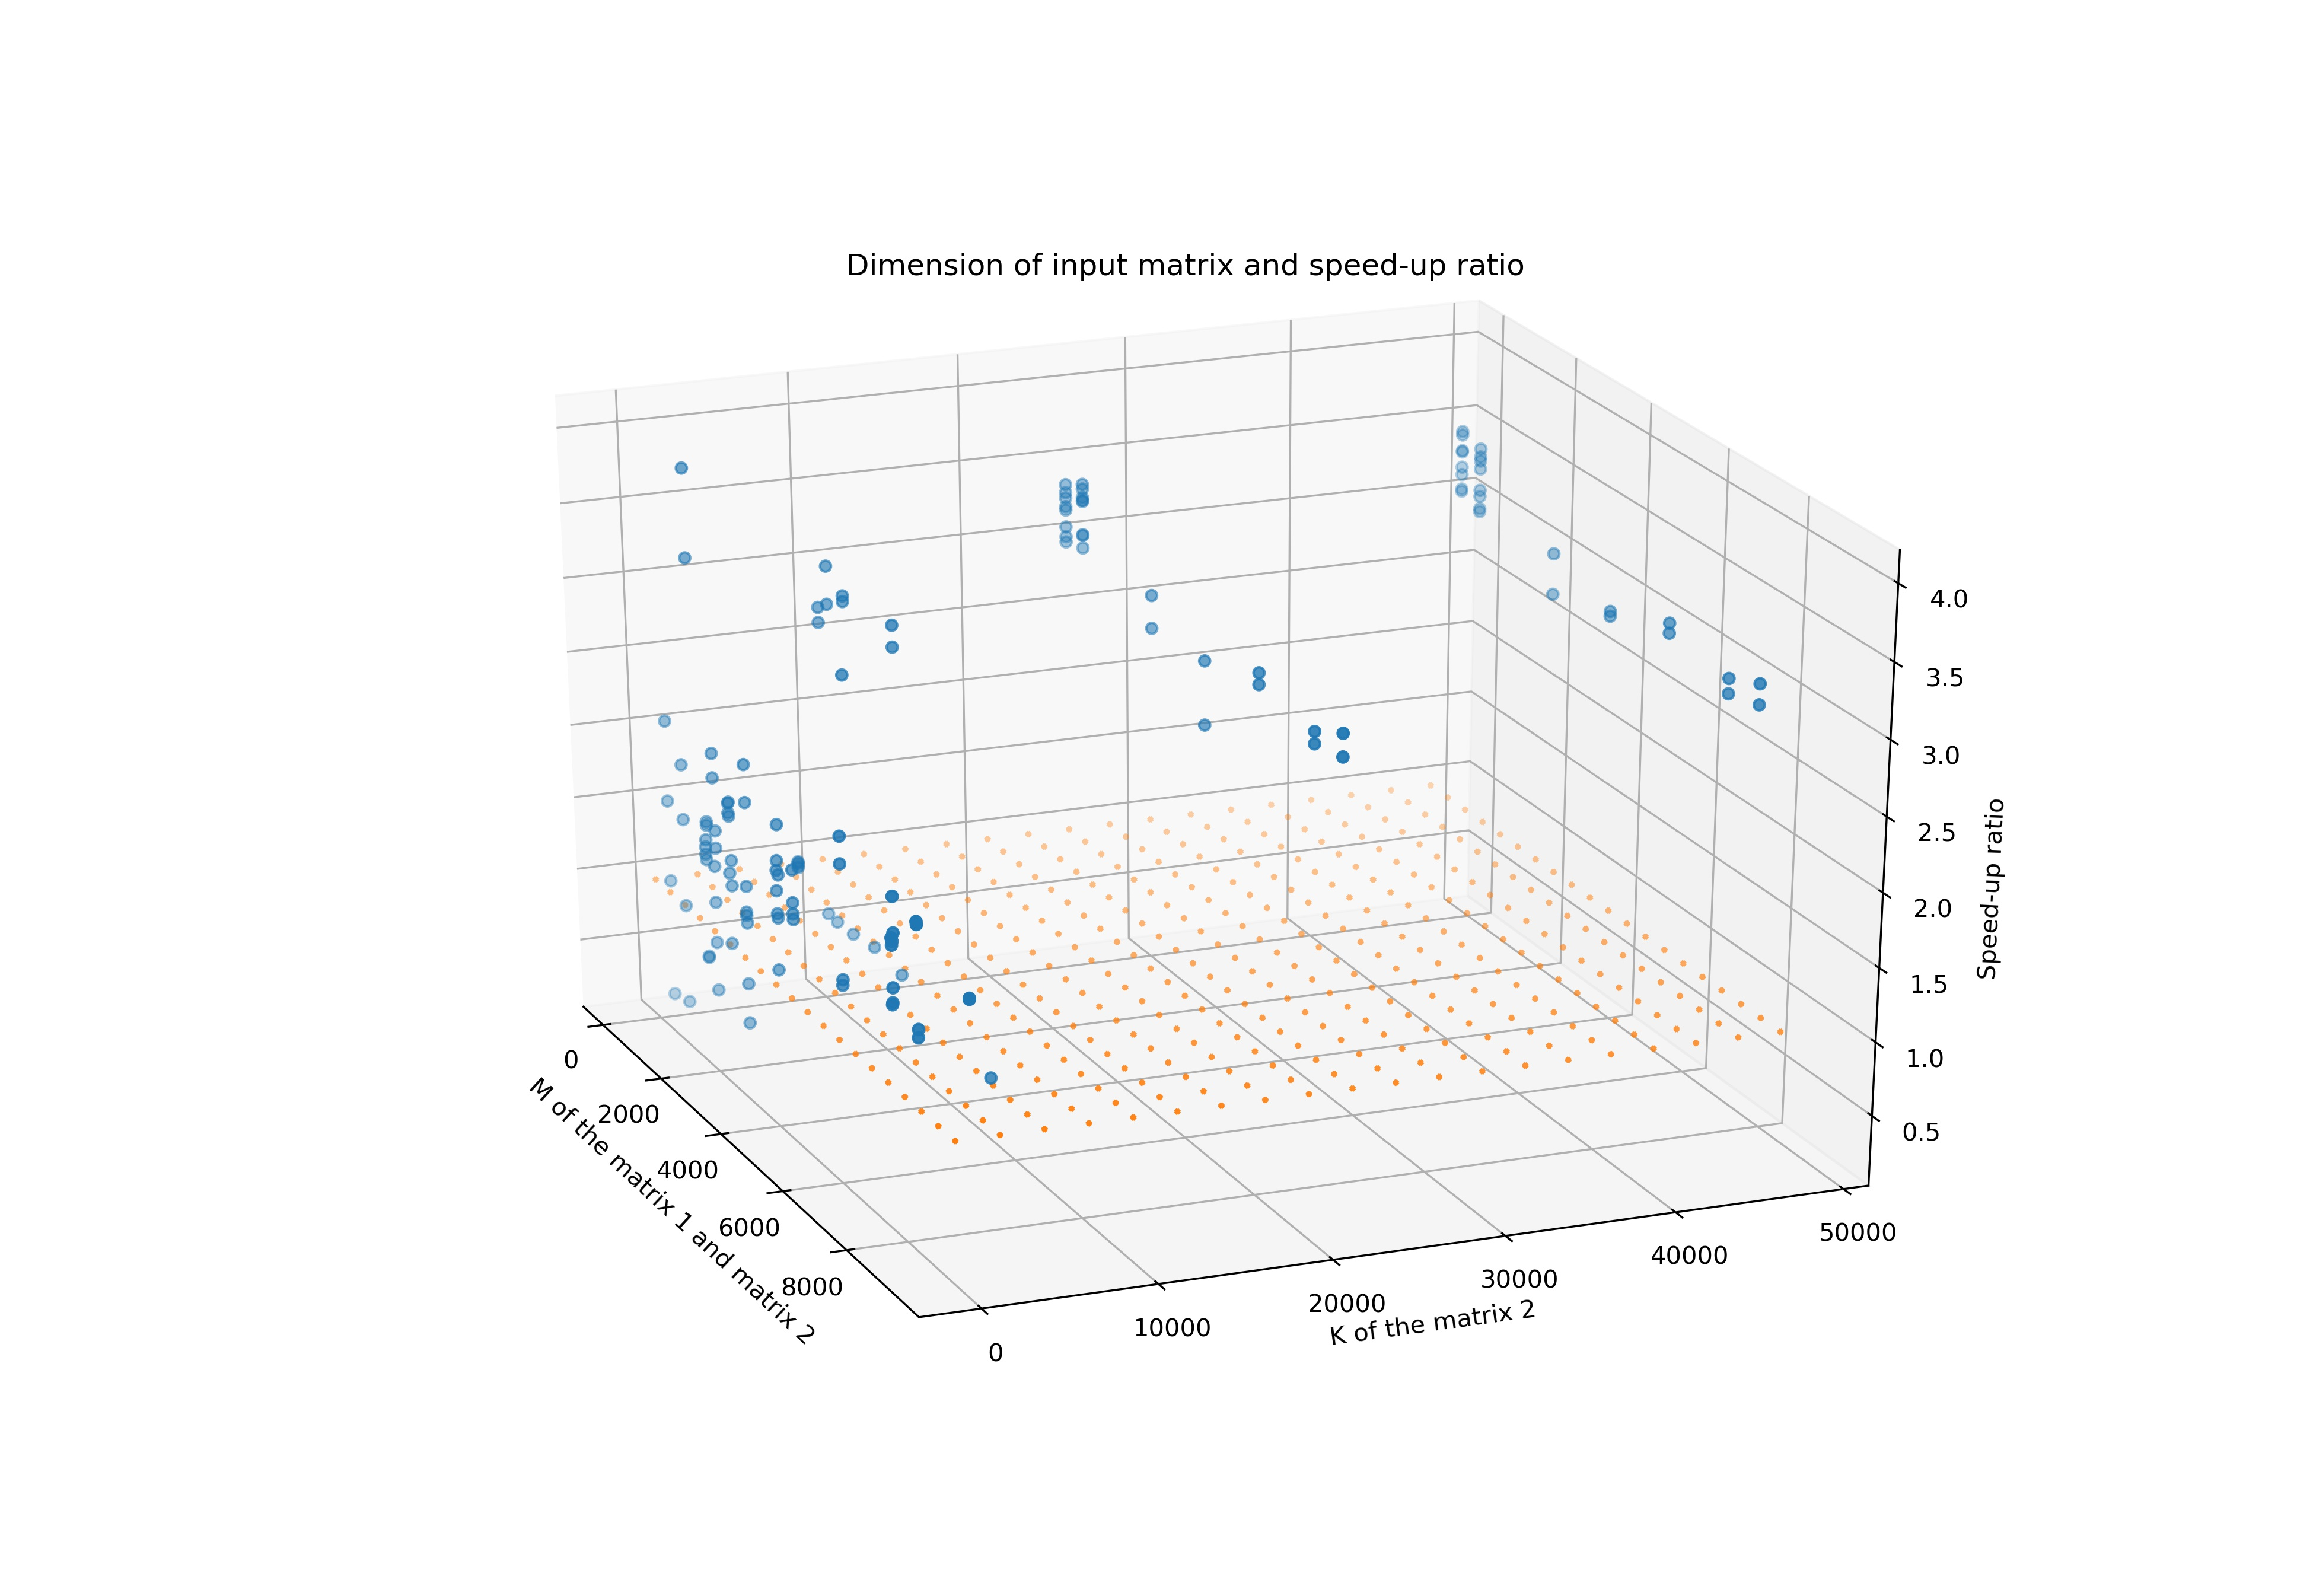
\includegraphics[width=7.5cm]{figures/GEMM_MK.jpg}
	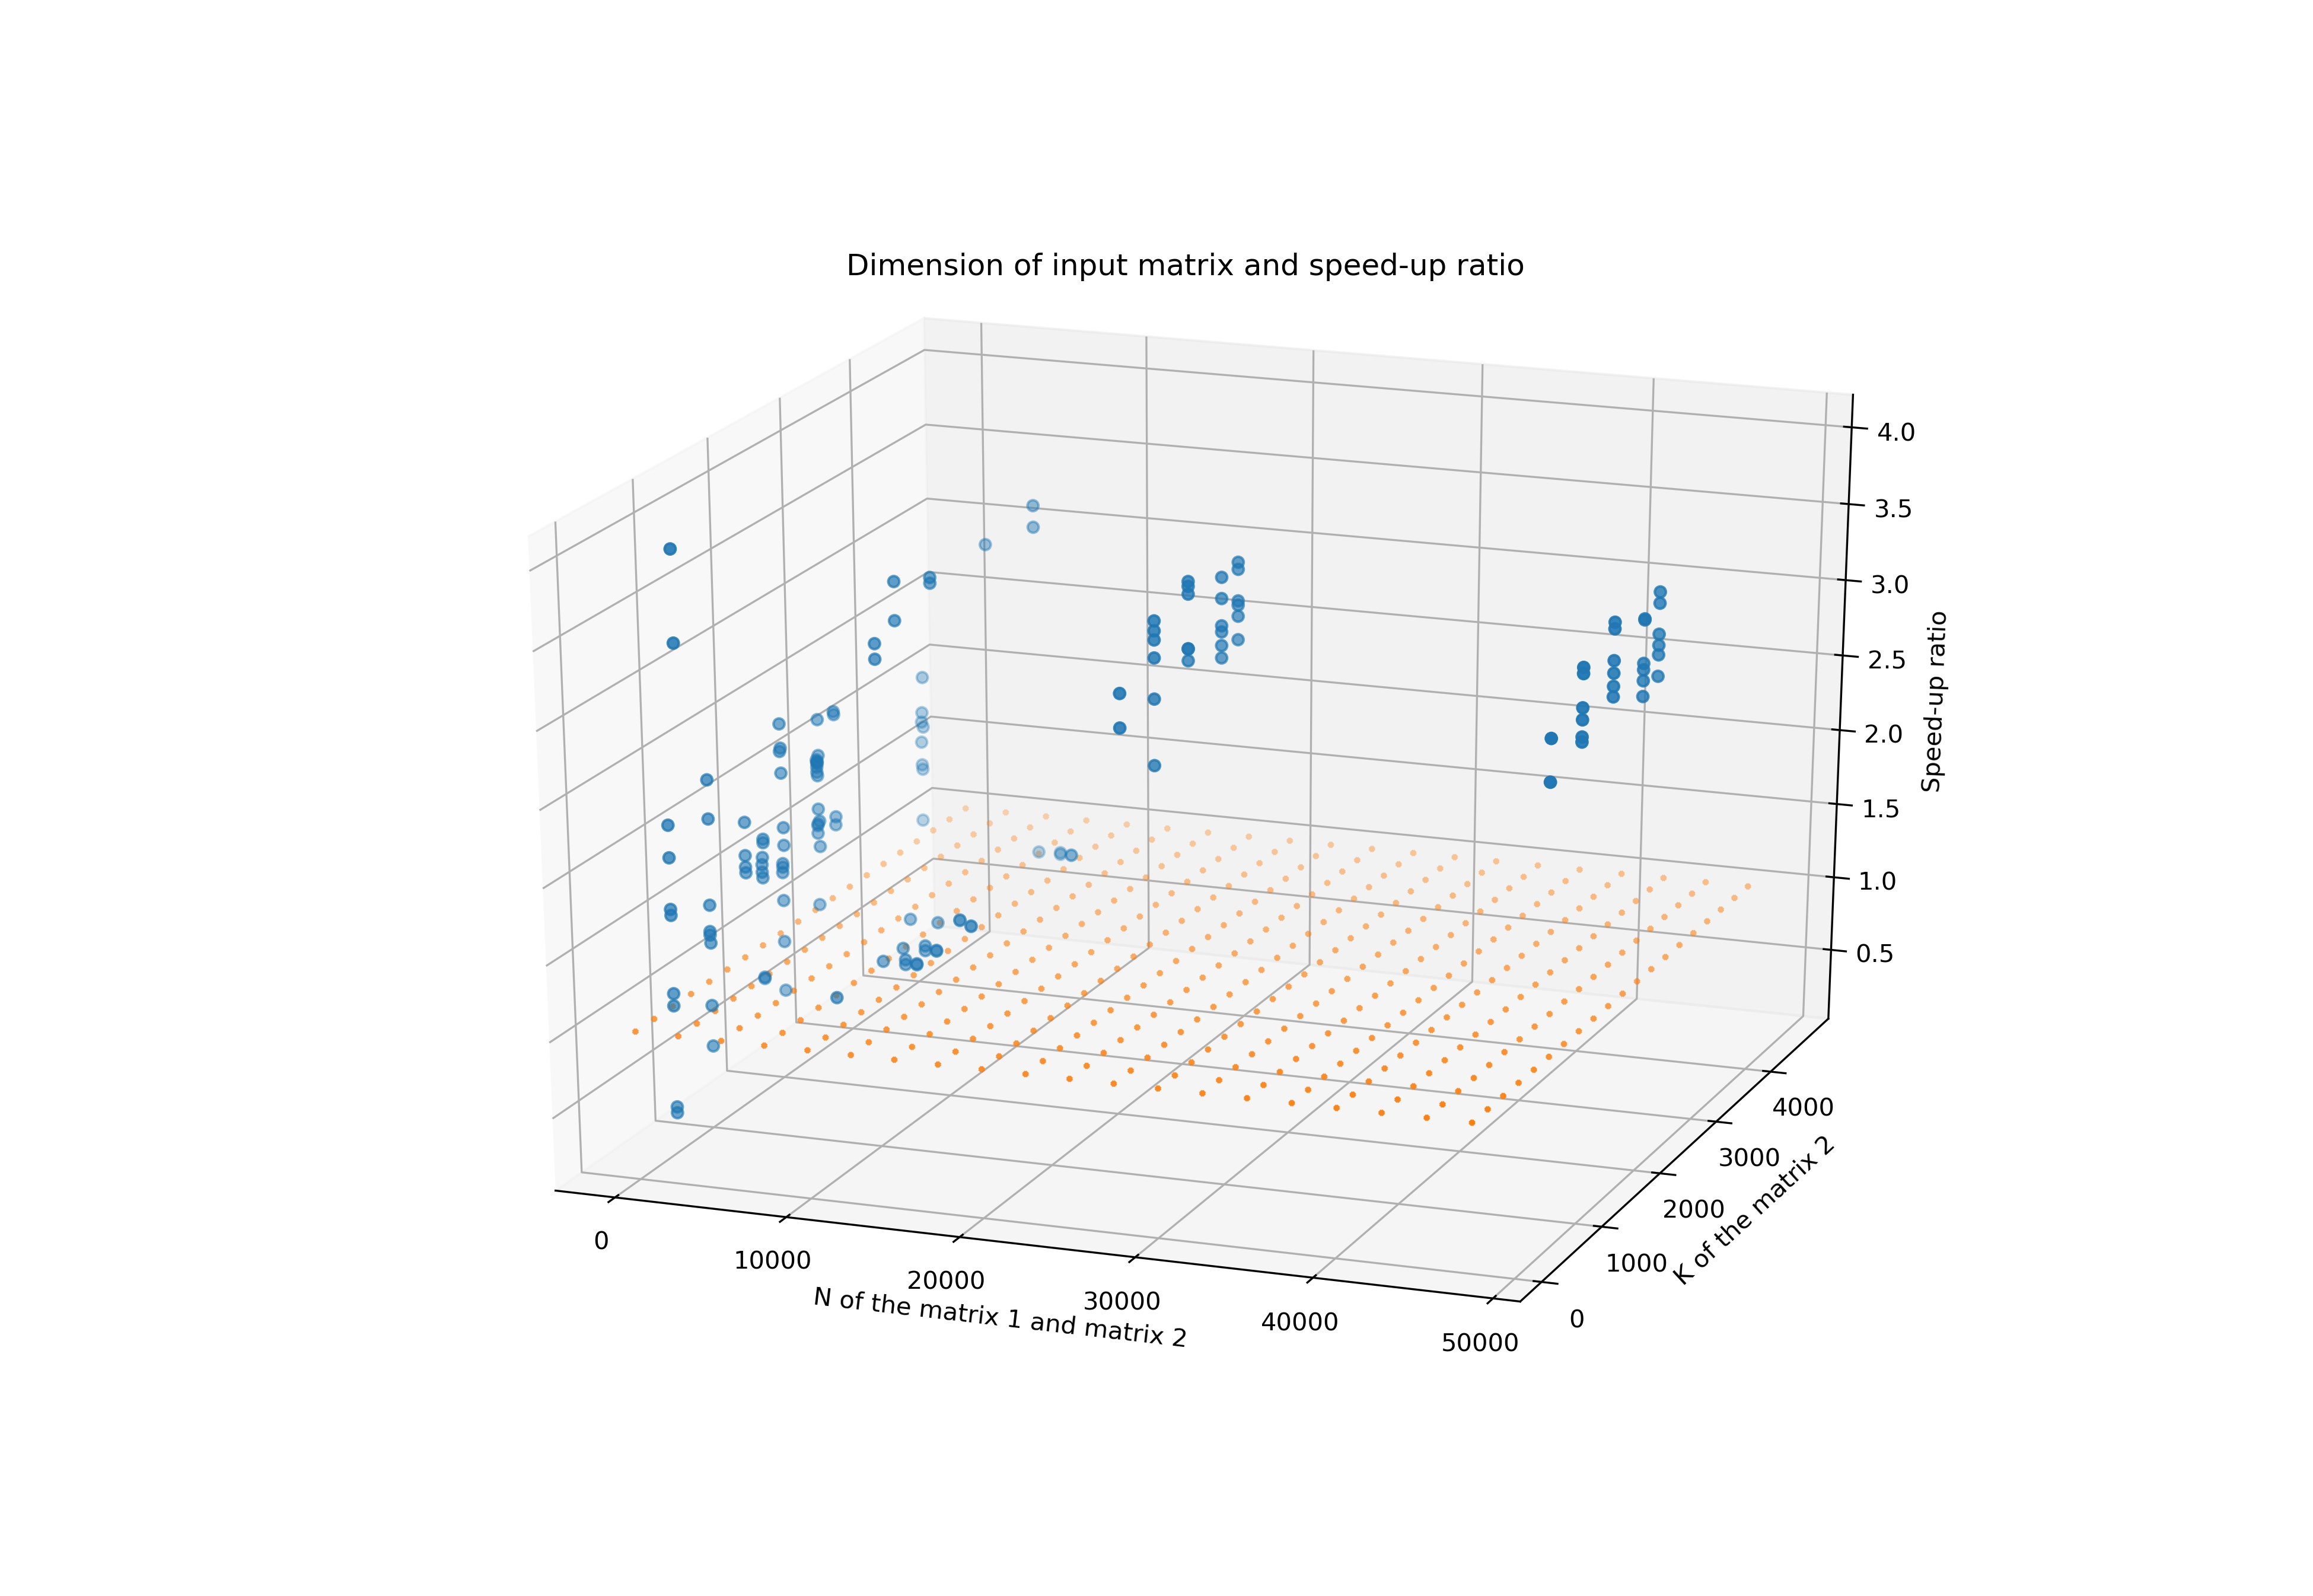
\includegraphics[width=7.5cm]{figures/GEMM_NK.jpg}\\
	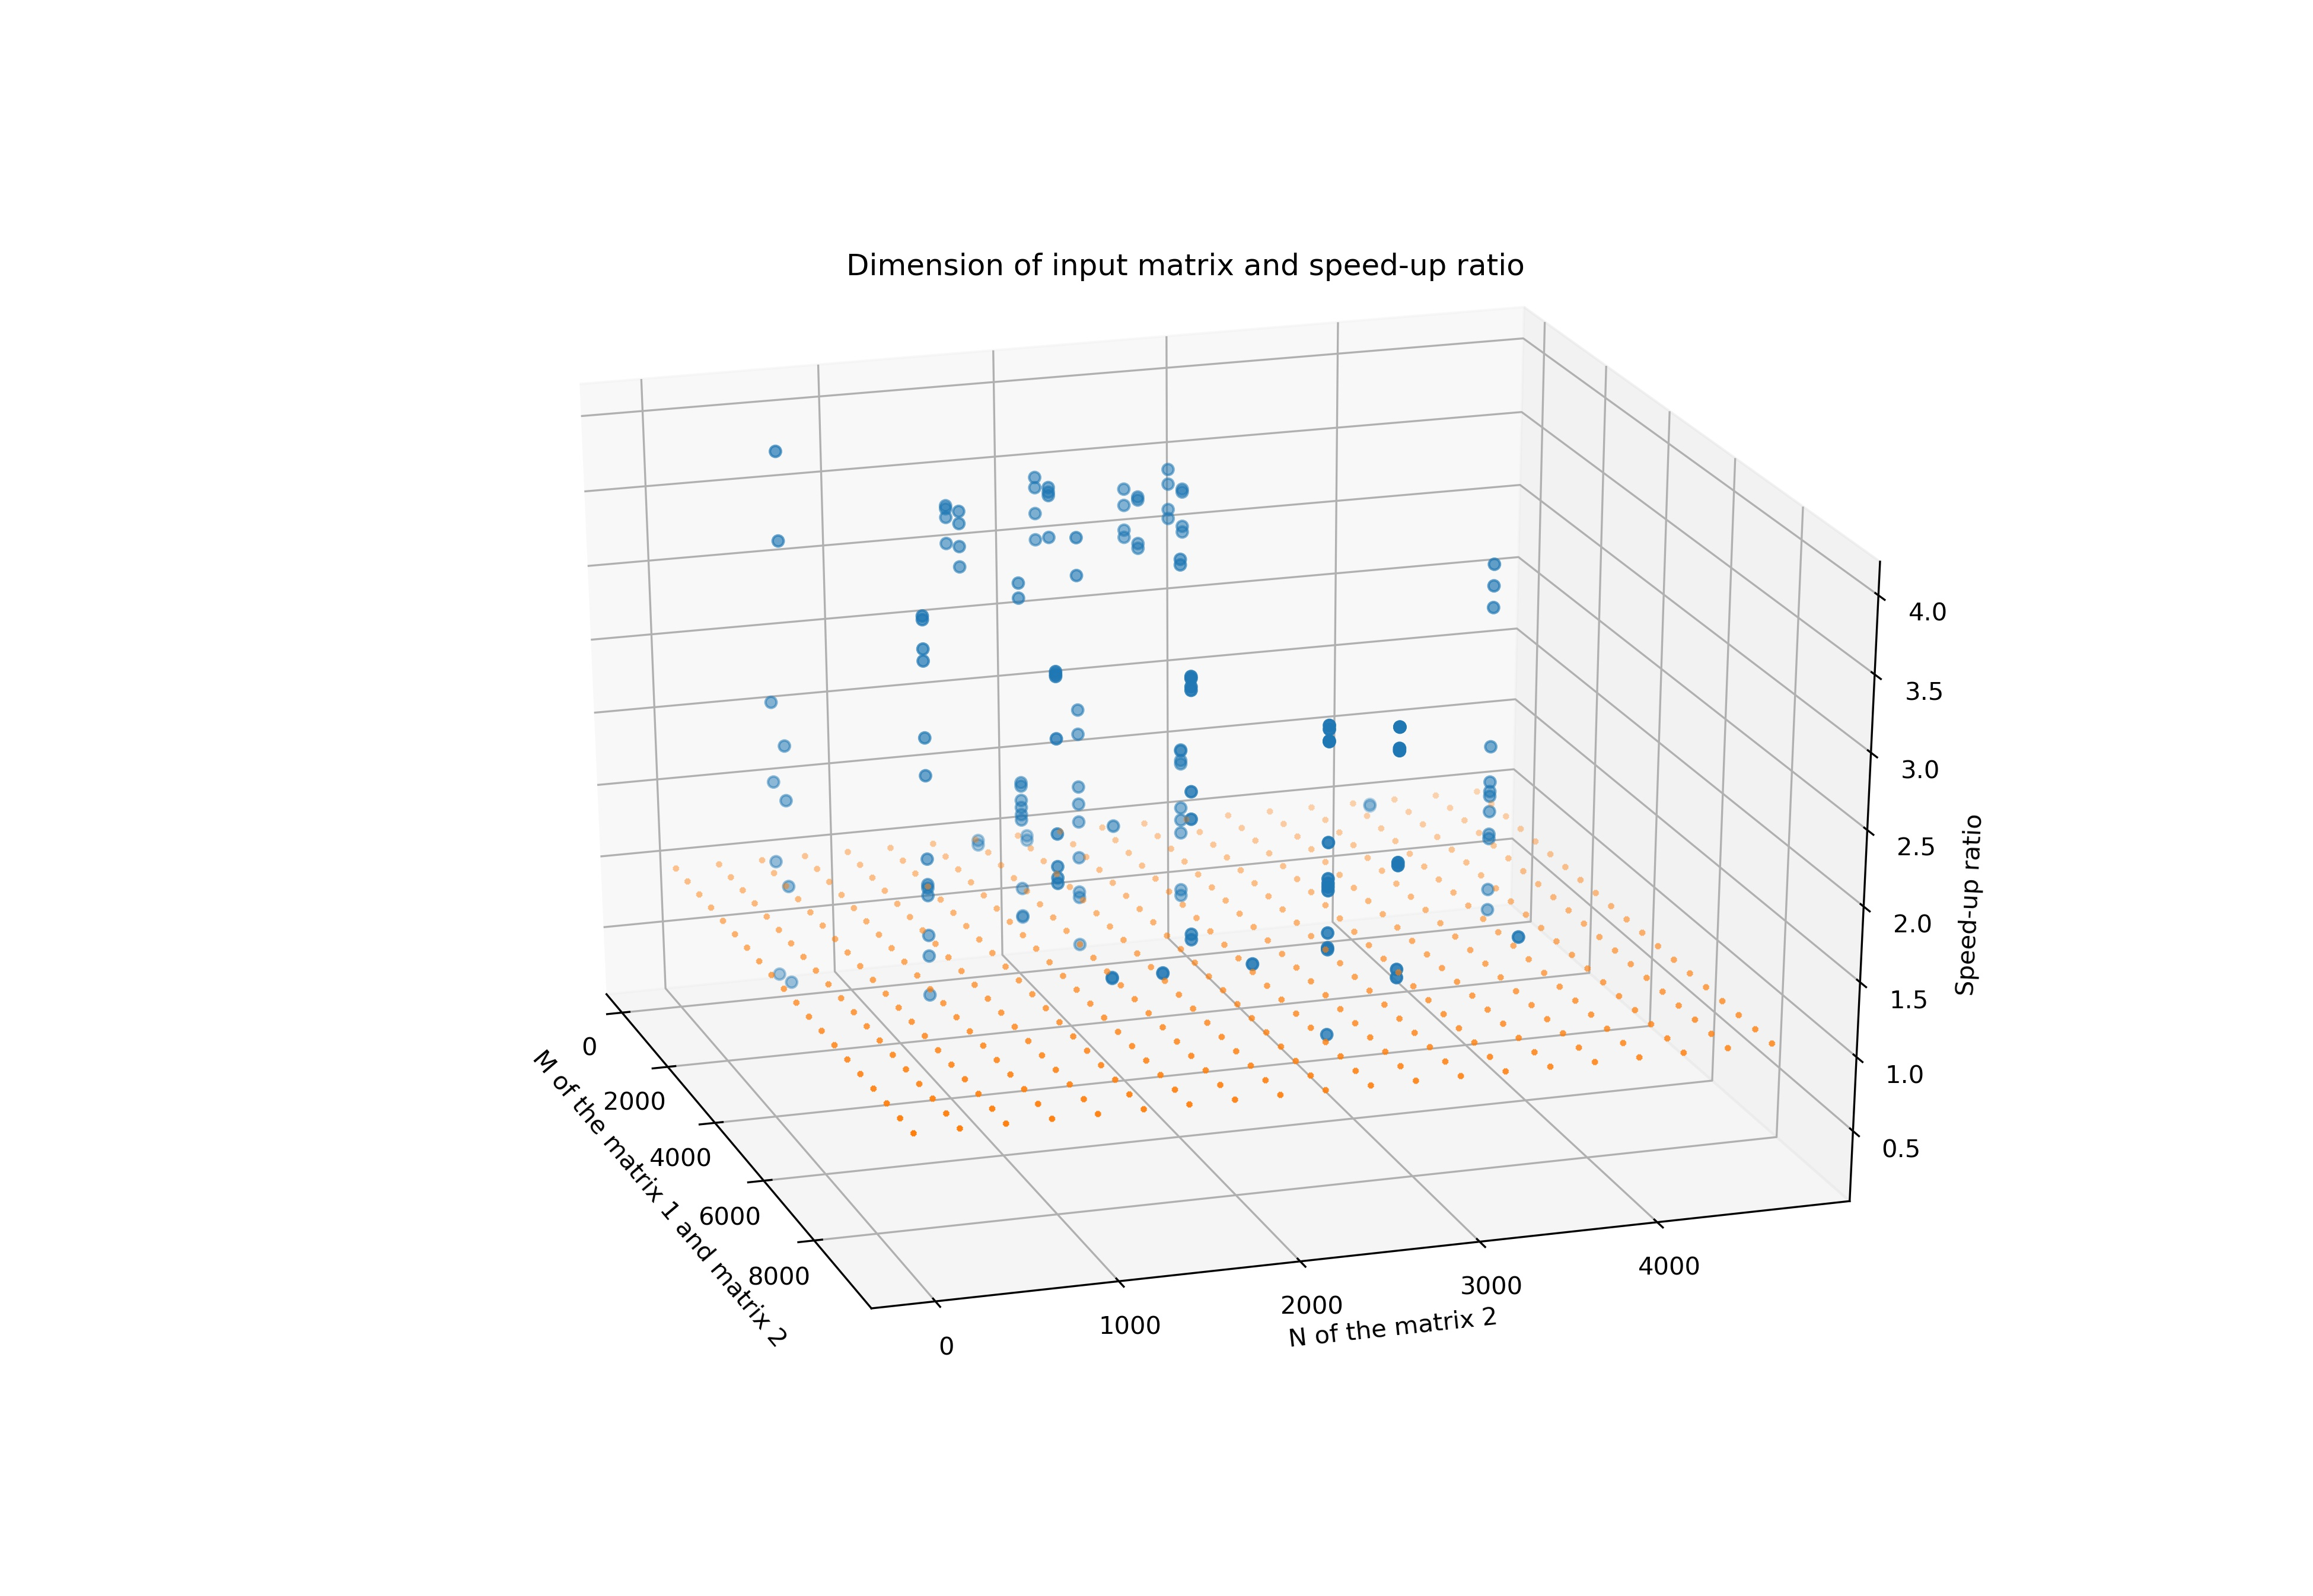
\includegraphics[width=7.5cm]{figures/GEMM_MN.jpg}
	\renewcommand{\thefigure}{\arabic{section}-\arabic{figure} }
	\renewcommand{\figurename}{图}
	\caption{输入矩阵维度与加速比的关系}
	\addtocounter{figure}{-1}
	\renewcommand{\thefigure}{\arabic{section}-\arabic{figure} }
	\renewcommand{\figurename}{Figure}
	\caption{Relationship of input matrix dimension and speed-up ratio}
	\label{Fig-MNKRatio}
\end{figure}
\begin{figure}
	\centering
	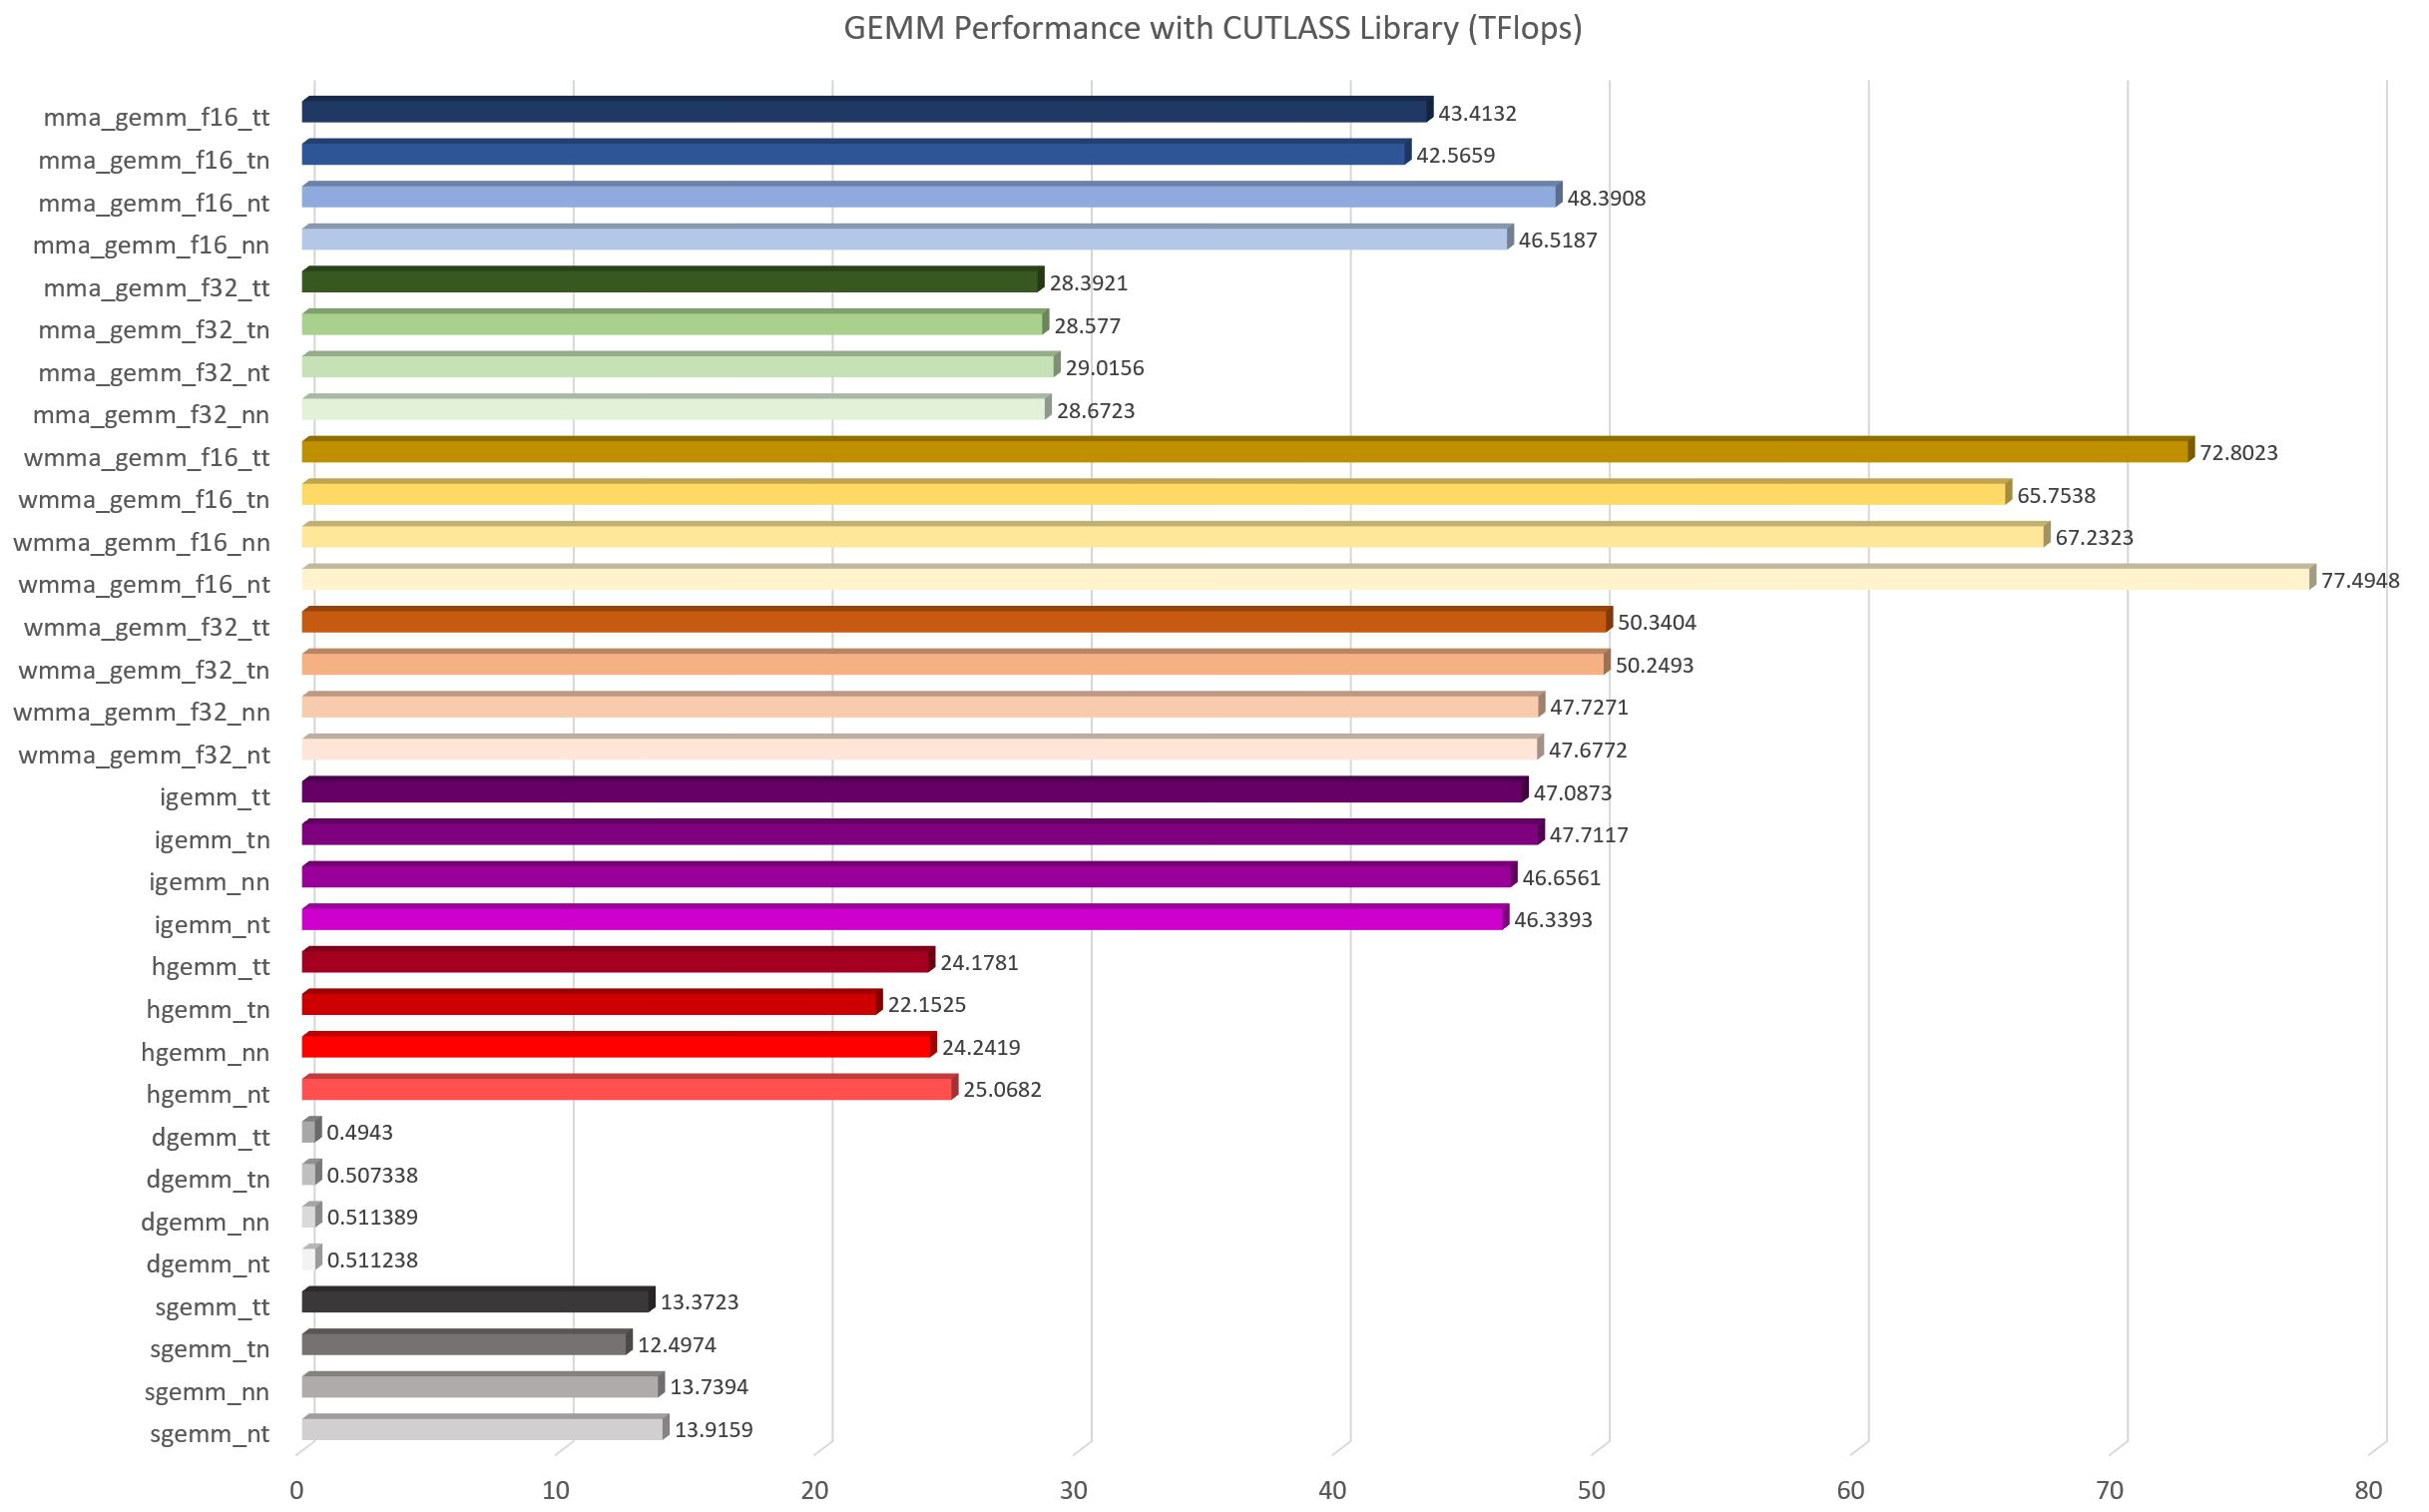
\includegraphics[width=15cm]{figures/CUTLASSGEMM.jpg}
	\renewcommand{\thefigure}{\arabic{section}-\arabic{figure} }
	\renewcommand{\figurename}{图}
	\caption{使用模板库测得的GEMM性能}
	\addtocounter{figure}{-1}
	\renewcommand{\thefigure}{\arabic{section}-\arabic{figure} }
	\renewcommand{\figurename}{Figure}
	\caption{GEMM Performance with CUTLASS}
	\label{Fig-GEMM-CUTLASS}
\end{figure}
\subparagraph{结果分析}
\paragraph{矩阵乘法运算}
\subparagraph{实验结果}
\subparagraph{结果分析}
\paragraph{卷积运算}
\subparagraph{实验结果}
\subparagraph{结果分析}
\paragraph{神经网络推理}
\subparagraph{实验结果}
\subparagraph{结果分析}
\subsubsection{基于CUDA源码的应用}
\paragraph{卷积神经网络}
\subparagraph{实验结果}
\subparagraph{结果分析}
\paragraph{并行支持向量机}
\subparagraph{实验结果}
\subparagraph{结果分析}
\subsubsection{基于TensorFlow框架的应用}
\subparagraph{实验结果}
\subparagraph{结果分析} %正文第三章
\newpage
\section{总结与展望}
\setcounter{table}{0}
\setcounter{figure}{0}
\par 本文主要通过自底向上的方式对NVIDIA最近发布的新架构硬件(伏特、图灵架构)在机器学习应用中的性能提升进行了评估,其中在新架构中新加入的张量核心(Tensor Core)是本文考察的重点,并根据评估结果给出了编程建议,以及对于下一代硬件的一些合理设想。
\par 在正式评估之前,本文对基于CUDA的GPU编程模型进行了简要介绍,其中包含CUDA应用程序的编写步骤、调用方式、内存模型等,同时还对中间层的PTX代码进行了简要介绍,这些知识对于后文性能分析部分有较大的帮助。接下来本文便从三个层级对基于CUDA的机器学习应用在新架构硬件上的性能提升幅度进行了评估。
\par 首先,本文涉及的最低层面便是用途单一、专为评估绝对性能设计的简单应用进行基准测试,这些应用大部分是NVIDIA官方发布的测试用例。这些测试用例涵盖混合矩阵运算(GEMM)、矩阵乘法、卷积核神经网络推理。根据实验得到的结果,在混合矩阵运算(GEMM)方面,新架构硬件能在操作数形状、尺寸与硬件参数、调用特征较为匹配的情况下取得大幅度的性能提升,而这些显著的性能提升是采用“用精度换速度”的策略,计算时数据精度均为FP16/INT8等低于传统的精度;然而在不匹配的情况下,性能下降极为明显。在矩阵乘法方面,我们评估了cuBLAS在新架构上的性能提升,结果是在所有情况下使用cuBLAS进行矩阵乘法运算优势都极为明显,且不依赖于操作数的形状、尺寸。在卷积运算方面,基于混合矩阵运算的卷积计算在新架构上相对于原有的基于快速傅里叶变换的计算方法在大规模输入时提升明显,且精度更高;然而在输入规模较小时,使用纹理内存进行直接计算占绝对优势。考虑到目前许多神经网络中的卷积计算的图像规模多为100-1000数量级,在该数量级上使用纹理内存进行直接计算的方法性能较强,实际应用中应考虑这种方法。以上三种大多是在网络训练阶段涉及的计算,而在网络推理阶段,本文尝试了一种新的模式,即使用TensorRT对训练好的网络结构进行优化并在目标硬件上进行推理。尽管TensorRT目前仅能运行于特定硬件,但是根据本文的实验,使用TensorRT能为网络推理带来极大的吞吐量提升。
\par 在完成基准测试之后,本文移步基于CUDA源码构建的机器学习应用。在该部分中本文分为深度学习应用和传统机器学习应用。深度学习应用选用了结构较为简单的卷积神经网络,而传统机器学习应用选择了支持向量机。在卷积神经网络部分,本文将计算分为前向传播,反向传播更新连接参数,反向传播更新卷积核参数三个部分,分别考察新架构对于这三个部分的提升幅度。实验结果令人意外,除去前向传播中新架构能带来30\%-50\%的提升外,另两个部分中开启新架构甚至会降低性能。其原因为反向传播部分多为梯度计算,能使用混合矩阵计算(GEMM)从而利用到Tensor Core的部分较少,而开启Tensor Core又会对调度、同步、访存和其他指令的发射带来影响,故反向部分会造成性能下降。而前向传播部分由于卷积核、步进、填充的存在,无法保证每一层操作数的形状都能适用于Tensor Core,故提升幅度极为有限。值得注意的是,通过将卷积操作更换为第二章中提到的纹理内存方式,总体性能得到了一定的提升。在支持向量机部分,本文则根据支持向量机输入矩阵较为稀疏的特征,分别考察了使用专为稀疏矩阵设计的API和使用Tensor Core的API进行评估,实验结果表明在数据量较大时,特征矩阵会愈稀疏,专为稀疏矩阵设计的API性能较好,而数据量较小时,仍然是使用Tensor Core的API性能较好。
\par 之后,本文对基于TensorFlow-GPU框架的应用进行评估。在这一部分我们搭建了一个简单的基于TensorFlow-GPU的卷积神经网络,目的在于考察在最贴近真实应用场景时如何尽可能利用新硬件提升性能。本文从神经网络的超参数、网络结构、卷积计算方式、数据精度和推理等方面进行考察;结果发现增加网络的批大小能带来显著的训练速度提升,但是过大的批会导致网络准确度下降,实际应用中应权衡这两点;而由于输入的图片尺寸较小,本文通过修改Tensor Flow源代码,将内建的卷积计算方式更换为使用纹理内存的直接方式后,取得了较为明显的提升且网络准确度仍然维持在较高的水平,然而由于这种方式局限大,且更改源码需要重新编译、安装,这个过程极为麻烦,故实际应用中不推荐对源码进行更改;在数据精度方面,使用FP16/INT8代替FP32并不会对网络总体准确度带来太大的下降,而在训练速度上提升很明显,实际应用中在准确度要求不高的情况下可以考虑用低精度数据替换;网络结构方面,将卷积核大小改为适合Tensor Core计算的形状能给训练速度带来一定提升,但是会极大降低网络准确度,实际应用中不推荐使用。最后,本文使用TensorRT对训练好的模型进行推理,在延迟方面有40%-50%的提升,故涉及到需要部署在设备上、对响应时间有要求的应用,应使用TensorRT进行优化。
\par 通过以上实验,可以总结出新架构的确能在特定情况下为机器学习中大量存在的矩阵混合运算带来明显的性能提升,从而提升总体机器学习应用的性能,然而目前为止,硬件仍然对输入、结构等较为敏感。且有些情况下仍然有性能更高的传统方式。所以在实际编码时,应根据问题规模、算法、结构、数据分布等方面合适选择不同方法,而不是一味使用新硬件提供的方法。
\par 最后,根据实验中发现的一些问题,本文做出了合理地设想,如计算规模更大、跨越多个线程束执行混合矩阵运算的新指令,以单个线程为粒度的同步机制等;这些设想是否会应验,或者在一定程度上实现,只能交给时间去判断,这里仅仅提出我们的设想供启发。
 %正文第四章
% \section{注释与引用}这节用来展示注释与引用。

\subsection{注释——脚注与尾注}
\subsubsection{脚注}
\par 这里是脚注测试\footnote{1111111111}这里是脚注测试这里是脚注测试这里是脚注测试\footnote{2222222222}这里是脚注测试这里是脚注测试这里是脚注测试这里是脚注测试这里是脚注测试这里是脚注测试这里是脚注测试这里是脚注测试这里是脚注测试这里是脚注测试这里是脚注测试这里是脚注测试这里是脚注测试这里是脚注测试这里是脚注测试\footnote{3333333333}这里是脚注测试这里是脚注测试这里是脚注测试这里是脚注测试这里是脚注测试这里是脚注测试这里是脚注测试这里是脚注测试这里是脚注测试这里是脚注测试这里是脚注测试这里是脚注测试

\textcolor{red}{\textbf{\uline{注意!正如这份演示中所出现的情况,若该页(也就是本文档中的前一页)剩余空间不大,不足以显示足够多的文档与脚注,那么该段文字就会被移至下一页而留下空白。目前我们尚未找到解决的方法,所以如果遇到了这个问题,请修改排版,以留下足够大的空间。}}}

\subsubsection{尾注}
\par 这里是尾注测试\endnote{伴随着互联网的发展以及新的网络应用的出现,互联网用户由单纯的“读”网页,向“读、写”网页,共同建设互联网发展,由此网上产生了大量带有用户主观感情的数据,从这些带...}这里是尾注测试这里是尾注测试这里是尾注测试这里是尾注测试\endnote{尾注测试2}这里是尾注测试这里是尾注测试这里是尾注测试这里是尾注测试这里是尾注测试这里是尾注测试这里是尾注测试这里是尾注测试这里是尾注测试这里是尾注测试这里是尾注测试这里是尾注测试这里是尾注测试这里是尾注测试这里是尾注测试\endnote{尾注测试3}这里是尾注测试这里是尾注测试这里是尾注测试这里是尾注测试这里是尾注测试这里是尾注测试这里是尾注测试这里是尾注测试这里是尾注测试

\par \textcolor{red}{\textbf{\uline{注意!endnotes宏包并不支持hyperref,也就是无法通过点击文中尾注标号以跳转到尾注。当然,这在打印出来的文档中并不会造成任何影响。}}}
\par \textcolor{blue}{\textbf{\uline{提示:尾注出现在全文最后。为了区分脚注与尾注的编号,我们在尾注编号前加上了“尾注”二字。}}}

\subsection{交叉引用}
\par 本模板使用cleveref宏包来进行交叉引用。使用的指令为$\backslash$cref$\{$label$\}$。例子如下:
\par 由\cref{thm2_1}我们可以知道XXXXXXXX。
\par 由\cref{lem2_2}我们可以知道XXXXXXXX。
\par 请注意,label是需要手工设置的,一般将label放在你需要引用的环境内即可(具体可见SectionB.tex)。

\subsection{文献引用的演示}
\par 本模板使用biblatex进行文献管理,这是一套相对较新的系统。另外,使用了hushidong制作的符合gb7714-2015标准的biblatex样式。在此对他的工作表示感谢,要完成这样的样式非常不容易。本模板中gb7714-2015.bbx与gb7714-2015.cbx即为他的作品,在这里打包发布以便使用。
\par 默认的bib文件位于~/reference/thesis-ref.bib,内容是由Wang Tianshu制作,在此仅作演示之用。关于bib文件的编写与管理请自行查找相关教程。
\par 下方的演示已经给出了正文中引用文献的基本方法,这与传统的cite命令是类似的。如有更多需求,请至\url{https://github.com/hushidong/biblatex-gb7714-2015}查找相关资料。
\par \textcolor{blue}{\textbf{\uline{本模板使用parencite而不是cite命令,因为这样能与脚注所产生编号进行区分。当然,如果你没有脚注或尾注,那么cite命令也是推荐使用的。}}}

 %正文第五章

%\theendnotes %尾注(若没有尾注请将本行删除)
\ClearPageStyle

%生成参考文献
\phantomsection
\addcontentsline{toc}{section}{参考文献}
\printbibliography[title={\sffamily \zihao {-3}参考文献}] 
\ClearPageStyle

%\makeapdx %生成附录
%\ClearPageStyle

\makeacknowledgement %生成感谢

\end{document}
